%%%%%%%%%%%%%%%%%%%%%%%%%%%%%%%%%%%%%%%%%
% The Legrand Orange Book
% LaTeX Template
% Version 2.0 (9/2/15)
%
% This template has been downloaded from:
% http://www.LaTeXTemplates.com
%
% Mathias Legrand (legrand.mathias@gmail.com) with modifications by:
% Vel (vel@latextemplates.com)
%
% License:
% CC BY-NC-SA 3.0 (http://creativecommons.org/licenses/by-nc-sa/3.0/)
%
% Compiling this template:
% This template uses biber for its bibliography and makeindex for its index.
% When you first open the template, compile it from the command line with the 
% commands below to make sure your LaTeX distribution is configured correctly:
%
% 1) pdflatex main
% 2) makeindex main.idx -s StyleInd.ist
% 3) biber main
% 4) pdflatex main x 2
%
% After this, when you wish to update the bibliography/index use the appropriate
% command above and make sure to compile with pdflatex several times 
% afterwards to propagate your changes to the document.
%
% This template also uses a number of packages which may need to be
% updated to the newest versions for the template to compile. It is strongly
% recommended you update your LaTeX distribution if you have any
% compilation errors.
%
% Important note:
% Chapter heading images should have a 2:1 width:height ratio,
% e.g. 920px width and 460px height.
%
%%%%%%%%%%%%%%%%%%%%%%%%%%%%%%%%%%%%%%%%%

%----------------------------------------------------------------------------------------
%	PACKAGES AND OTHER DOCUMENT CONFIGURATIONS
%----------------------------------------------------------------------------------------

\documentclass[11pt,fleqn]{book} % Default font size and left-justified equations


\usepackage{mathrsfs}
\usepackage{amsbsy}



\newcommand{\indep}{\rotatebox[origin=c]{90}{$\models$}}

%----------------------------------------------------------------------------------------

%fdlkjadlkjdfsal;kjafds;lkjafsd;lkjfsad

%%%%%%%%%%%%%%%%%%%%%%%%%%%%%%%%%%%%%%%%%
% The Legrand Orange Book
% Structural Definitions File
% Version 2.0 (9/2/15)
%
% Original author:
% Mathias Legrand (legrand.mathias@gmail.com) with modifications by:
% Vel (vel@latextemplates.com)
% 
% This file has been downloaded from:
% http://www.LaTeXTemplates.com
%
% License:
% CC BY-NC-SA 3.0 (http://creativecommons.org/licenses/by-nc-sa/3.0/)
%
%%%%%%%%%%%%%%%%%%%%%%%%%%%%%%%%%%%%%%%%%

%----------------------------------------------------------------------------------------
%	VARIOUS REQUIRED PACKAGES AND CONFIGURATIONS
%----------------------------------------------------------------------------------------

\usepackage[top=3cm,bottom=3cm,left=3cm,right=3cm,headsep=10pt,a4paper]{geometry} % Page margins

\usepackage{graphicx} % Required for including pictures
\graphicspath{{Pictures/}} % Specifies the directory where pictures are stored

\usepackage{lipsum} % Inserts dummy text

\usepackage{tikz} % Required for drawing custom shapes

\usepackage[english]{babel} % English language/hyphenation

\usepackage{enumitem} % Customize lists
\setlist{nolistsep} % Reduce spacing between bullet points and numbered lists

\usepackage{booktabs} % Required for nicer horizontal rules in tables

\usepackage{xcolor} % Required for specifying colors by name
\definecolor{ocre}{RGB}{243,102,25} % Define the orange color used for highlighting throughout the book

%----------------------------------------------------------------------------------------
%	FONTS
%----------------------------------------------------------------------------------------

\usepackage{avant} % Use the Avantgarde font for headings
%\usepackage{times} % Use the Times font for headings
\usepackage{mathptmx} % Use the Adobe Times Roman as the default text font together with math symbols from the Sym­bol, Chancery and Com­puter Modern fonts

\usepackage{microtype} % Slightly tweak font spacing for aesthetics
\usepackage[utf8]{inputenc} % Required for including letters with accents
\usepackage[T1]{fontenc} % Use 8-bit encoding that has 256 glyphs

%----------------------------------------------------------------------------------------
%	BIBLIOGRAPHY AND INDEX
%----------------------------------------------------------------------------------------

\usepackage[style=alphabetic,citestyle=numeric,sorting=nyt,sortcites=true,autopunct=true,babel=hyphen,hyperref=true,abbreviate=false,backref=true,backend=biber]{biblatex}
\addbibresource{bibliography.bib} % BibTeX bibliography file
\defbibheading{bibempty}{}

\usepackage{calc} % For simpler calculation - used for spacing the index letter headings correctly
\usepackage{makeidx} % Required to make an index
\makeindex % Tells LaTeX to create the files required for indexing

%----------------------------------------------------------------------------------------
%	MAIN TABLE OF CONTENTS
%----------------------------------------------------------------------------------------

\usepackage{titletoc} % Required for manipulating the table of contents

\contentsmargin{0cm} % Removes the default margin

% Part text styling
\titlecontents{part}[0cm]
{\addvspace{20pt}\centering\large\bfseries}
{}
{}
{}

% Chapter text styling
\titlecontents{chapter}[1.25cm] % Indentation
{\addvspace{12pt}\large\sffamily\bfseries} % Spacing and font options for chapters
{\color{ocre!60}\contentslabel[\Large\thecontentslabel]{1.25cm}\color{ocre}} % Chapter number
{\color{ocre}}  
{\color{ocre!60}\normalsize\;\titlerule*[.5pc]{.}\;\thecontentspage} % Page number

% Section text styling
\titlecontents{section}[1.25cm] % Indentation
{\addvspace{3pt}\sffamily\bfseries} % Spacing and font options for sections
{\contentslabel[\thecontentslabel]{1.25cm}} % Section number
{}
{\hfill\color{black}\thecontentspage} % Page number
[]

% Subsection text styling
\titlecontents{subsection}[1.25cm] % Indentation
{\addvspace{1pt}\sffamily\small} % Spacing and font options for subsections
{\contentslabel[\thecontentslabel]{1.25cm}} % Subsection number
{}
{\ \titlerule*[.5pc]{.}\;\thecontentspage} % Page number
[]

% List of figures
\titlecontents{figure}[0em]
{\addvspace{-5pt}\sffamily}
{\thecontentslabel\hspace*{1em}}
{}
{\ \titlerule*[.5pc]{.}\;\thecontentspage}
[]

% List of tables
\titlecontents{table}[0em]
{\addvspace{-5pt}\sffamily}
{\thecontentslabel\hspace*{1em}}
{}
{\ \titlerule*[.5pc]{.}\;\thecontentspage}
[]

%----------------------------------------------------------------------------------------
%	MINI TABLE OF CONTENTS IN PART HEADS
%----------------------------------------------------------------------------------------

% Chapter text styling
\titlecontents{lchapter}[0em] % Indenting
{\addvspace{15pt}\large\sffamily\bfseries} % Spacing and font options for chapters
{\color{ocre}\contentslabel[\Large\thecontentslabel]{1.25cm}\color{ocre}} % Chapter number
{}  
{\color{ocre}\normalsize\sffamily\bfseries\;\titlerule*[.5pc]{.}\;\thecontentspage} % Page number

% Section text styling
\titlecontents{lsection}[0em] % Indenting
{\sffamily\small} % Spacing and font options for sections
{\contentslabel[\thecontentslabel]{1.25cm}} % Section number
{}
{}

% Subsection text styling
\titlecontents{lsubsection}[.5em] % Indentation
{\normalfont\footnotesize\sffamily} % Font settings
{}
{}
{}

%----------------------------------------------------------------------------------------
%	PAGE HEADERS
%----------------------------------------------------------------------------------------

\usepackage{fancyhdr} % Required for header and footer configuration

\pagestyle{fancy}
\renewcommand{\chaptermark}[1]{\markboth{\sffamily\normalsize\bfseries\chaptername\ \thechapter.\ #1}{}} % Chapter text font settings
\renewcommand{\sectionmark}[1]{\markright{\sffamily\normalsize\thesection\hspace{5pt}#1}{}} % Section text font settings
\fancyhf{} \fancyhead[LE,RO]{\sffamily\normalsize\thepage} % Font setting for the page number in the header
\fancyhead[LO]{\rightmark} % Print the nearest section name on the left side of odd pages
\fancyhead[RE]{\leftmark} % Print the current chapter name on the right side of even pages
\renewcommand{\headrulewidth}{0.5pt} % Width of the rule under the header
\addtolength{\headheight}{2.5pt} % Increase the spacing around the header slightly
\renewcommand{\footrulewidth}{0pt} % Removes the rule in the footer
\fancypagestyle{plain}{\fancyhead{}\renewcommand{\headrulewidth}{0pt}} % Style for when a plain pagestyle is specified

% Removes the header from odd empty pages at the end of chapters
\makeatletter
\renewcommand{\cleardoublepage}{
\clearpage\ifodd\c@page\else
\hbox{}
\vspace*{\fill}
\thispagestyle{empty}
\newpage
\fi}

%----------------------------------------------------------------------------------------
%	THEOREM STYLES
%----------------------------------------------------------------------------------------

\usepackage{amsmath,amsfonts,amssymb,amsthm} % For math equations, theorems, symbols, etc

\newcommand{\intoo}[2]{\mathopen{]}#1\,;#2\mathclose{[}}
\newcommand{\ud}{\mathop{\mathrm{{}d}}\mathopen{}}
\newcommand{\intff}[2]{\mathopen{[}#1\,;#2\mathclose{]}}
\newtheorem{notation}{Notation}[chapter]

% Boxed/framed environments
\newtheoremstyle{ocrenumbox}% % Theorem style name
{0pt}% Space above
{0pt}% Space below
{\normalfont}% % Body font
{}% Indent amount
{\small\bf\sffamily\color{ocre}}% % Theorem head font
{\;}% Punctuation after theorem head
{0.25em}% Space after theorem head
{\small\sffamily\color{ocre}\thmname{#1}\nobreakspace\thmnumber{\@ifnotempty{#1}{}\@upn{#2}}% Theorem text (e.g. Theorem 2.1)
\thmnote{\nobreakspace\the\thm@notefont\sffamily\bfseries\color{black}---\nobreakspace#3.}} % Optional theorem note
\renewcommand{\qedsymbol}{$\blacksquare$}% Optional qed square

\newtheoremstyle{blacknumex}% Theorem style name
{5pt}% Space above
{5pt}% Space below
{\normalfont}% Body font
{} % Indent amount
{\small\bf\sffamily}% Theorem head font
{\;}% Punctuation after theorem head
{0.25em}% Space after theorem head
{\small\sffamily{\tiny\ensuremath{\blacksquare}}\nobreakspace\thmname{#1}\nobreakspace\thmnumber{\@ifnotempty{#1}{}\@upn{#2}}% Theorem text (e.g. Theorem 2.1)
\thmnote{\nobreakspace\the\thm@notefont\sffamily\bfseries---\nobreakspace#3.}}% Optional theorem note

\newtheoremstyle{blacknumbox} % Theorem style name
{0pt}% Space above
{0pt}% Space below
{\normalfont}% Body font
{}% Indent amount
{\small\bf\sffamily}% Theorem head font
{\;}% Punctuation after theorem head
{0.25em}% Space after theorem head
{\small\sffamily\thmname{#1}\nobreakspace\thmnumber{\@ifnotempty{#1}{}\@upn{#2}}% Theorem text (e.g. Theorem 2.1)
\thmnote{\nobreakspace\the\thm@notefont\sffamily\bfseries---\nobreakspace#3.}}% Optional theorem note

% Non-boxed/non-framed environments
\newtheoremstyle{ocrenum}% % Theorem style name
{5pt}% Space above
{5pt}% Space below
{\normalfont}% % Body font
{}% Indent amount
{\small\bf\sffamily\color{ocre}}% % Theorem head font
{\;}% Punctuation after theorem head
{0.25em}% Space after theorem head
{\small\sffamily\color{ocre}\thmname{#1}\nobreakspace\thmnumber{\@ifnotempty{#1}{}\@upn{#2}}% Theorem text (e.g. Theorem 2.1)
\thmnote{\nobreakspace\the\thm@notefont\sffamily\bfseries\color{black}---\nobreakspace#3.}} % Optional theorem note
\renewcommand{\qedsymbol}{$\blacksquare$}% Optional qed square
\makeatother

% Defines the theorem text style for each type of theorem to one of the three styles above
\newcounter{dummy} 
\numberwithin{dummy}{section}
\theoremstyle{ocrenumbox}
\newtheorem{theoremeT}[dummy]{Theorem}
\newtheorem{problem}{Problem}[chapter]
\newtheorem{exerciseT}{Exercise}[chapter]
\theoremstyle{blacknumex}
\newtheorem{exampleT}{Example}[chapter]
\theoremstyle{blacknumbox}
\newtheorem{vocabulary}{Vocabulary}[chapter]
\newtheorem{definitionT}{Definition}[section]
\newtheorem{corollaryT}[dummy]{Corollary}
\theoremstyle{ocrenum}
\newtheorem{proposition}[dummy]{Proposition}

%----------------------------------------------------------------------------------------
%	DEFINITION OF COLORED BOXES
%----------------------------------------------------------------------------------------

\RequirePackage[framemethod=default]{mdframed} % Required for creating the theorem, definition, exercise and corollary boxes

% Theorem box
\newmdenv[skipabove=7pt,
skipbelow=7pt,
backgroundcolor=black!5,
linecolor=ocre,
innerleftmargin=5pt,
innerrightmargin=5pt,
innertopmargin=5pt,
leftmargin=0cm,
rightmargin=0cm,
innerbottommargin=5pt]{tBox}

% Exercise box	  
\newmdenv[skipabove=7pt,
skipbelow=7pt,
rightline=false,
leftline=true,
topline=false,
bottomline=false,
backgroundcolor=ocre!10,
linecolor=ocre,
innerleftmargin=5pt,
innerrightmargin=5pt,
innertopmargin=5pt,
innerbottommargin=5pt,
leftmargin=0cm,
rightmargin=0cm,
linewidth=4pt]{eBox}	

% Definition box
\newmdenv[skipabove=7pt,
skipbelow=7pt,
rightline=false,
leftline=true,
topline=false,
bottomline=false,
linecolor=ocre,
innerleftmargin=5pt,
innerrightmargin=5pt,
innertopmargin=0pt,
leftmargin=0cm,
rightmargin=0cm,
linewidth=4pt,
innerbottommargin=0pt]{dBox}	

% Corollary box
\newmdenv[skipabove=7pt,
skipbelow=7pt,
rightline=false,
leftline=true,
topline=false,
bottomline=false,
linecolor=gray,
backgroundcolor=black!5,
innerleftmargin=5pt,
innerrightmargin=5pt,
innertopmargin=5pt,
leftmargin=0cm,
rightmargin=0cm,
linewidth=4pt,
innerbottommargin=5pt]{cBox}

% Creates an environment for each type of theorem and assigns it a theorem text style from the "Theorem Styles" section above and a colored box from above
\newenvironment{theorem}{\begin{tBox}\begin{theoremeT}}{\end{theoremeT}\end{tBox}}
\newenvironment{exercise}{\begin{eBox}\begin{exerciseT}}{\hfill{\color{ocre}\tiny\ensuremath{\blacksquare}}\end{exerciseT}\end{eBox}}				  
\newenvironment{definition}{\begin{dBox}\begin{definitionT}}{\end{definitionT}\end{dBox}}	
\newenvironment{example}{\begin{exampleT}}{\hfill{\tiny\ensuremath{\blacksquare}}\end{exampleT}}		
\newenvironment{corollary}{\begin{cBox}\begin{corollaryT}}{\end{corollaryT}\end{cBox}}	

%----------------------------------------------------------------------------------------
%	REMARK ENVIRONMENT
%----------------------------------------------------------------------------------------

\newenvironment{remark}{\par\vspace{10pt}\small % Vertical white space above the remark and smaller font size
\begin{list}{}{
\leftmargin=35pt % Indentation on the left
\rightmargin=25pt}\item\ignorespaces % Indentation on the right
\makebox[-2.5pt]{\begin{tikzpicture}[overlay]
\node[draw=ocre!60,line width=1pt,circle,fill=ocre!25,font=\sffamily\bfseries,inner sep=2pt,outer sep=0pt] at (-15pt,0pt){\textcolor{ocre}{R}};\end{tikzpicture}} % Orange R in a circle
\advance\baselineskip -1pt}{\end{list}\vskip5pt} % Tighter line spacing and white space after remark

%----------------------------------------------------------------------------------------
%	SECTION NUMBERING IN THE MARGIN
%----------------------------------------------------------------------------------------

\makeatletter
\renewcommand{\@seccntformat}[1]{\llap{\textcolor{ocre}{\csname the#1\endcsname}\hspace{1em}}}                    
\renewcommand{\section}{\@startsection{section}{1}{\z@}
{-4ex \@plus -1ex \@minus -.4ex}
{1ex \@plus.2ex }
{\normalfont\large\sffamily\bfseries}}
\renewcommand{\subsection}{\@startsection {subsection}{2}{\z@}
{-3ex \@plus -0.1ex \@minus -.4ex}
{0.5ex \@plus.2ex }
{\normalfont\sffamily\bfseries}}
\renewcommand{\subsubsection}{\@startsection {subsubsection}{3}{\z@}
{-2ex \@plus -0.1ex \@minus -.2ex}
{.2ex \@plus.2ex }
{\normalfont\small\sffamily\bfseries}}                        
\renewcommand\paragraph{\@startsection{paragraph}{4}{\z@}
{-2ex \@plus-.2ex \@minus .2ex}
{.1ex}
{\normalfont\small\sffamily\bfseries}}

%----------------------------------------------------------------------------------------
%	PART HEADINGS
%----------------------------------------------------------------------------------------

% numbered part in the table of contents
\newcommand{\@mypartnumtocformat}[2]{%
\setlength\fboxsep{0pt}%
\noindent\colorbox{ocre!20}{\strut\parbox[c][.7cm]{\ecart}{\color{ocre!70}\Large\sffamily\bfseries\centering#1}}\hskip\esp\colorbox{ocre!40}{\strut\parbox[c][.7cm]{\linewidth-\ecart-\esp}{\Large\sffamily\centering#2}}}%
%%%%%%%%%%%%%%%%%%%%%%%%%%%%%%%%%%
% unnumbered part in the table of contents
\newcommand{\@myparttocformat}[1]{%
\setlength\fboxsep{0pt}%
\noindent\colorbox{ocre!40}{\strut\parbox[c][.7cm]{\linewidth}{\Large\sffamily\centering#1}}}%
%%%%%%%%%%%%%%%%%%%%%%%%%%%%%%%%%%
\newlength\esp
\setlength\esp{4pt}
\newlength\ecart
\setlength\ecart{1.2cm-\esp}
\newcommand{\thepartimage}{}%
\newcommand{\partimage}[1]{\renewcommand{\thepartimage}{#1}}%
\def\@part[#1]#2{%
\ifnum \c@secnumdepth >-2\relax%
\refstepcounter{part}%
\addcontentsline{toc}{part}{\texorpdfstring{\protect\@mypartnumtocformat{\thepart}{#1}}{\partname~\thepart\ ---\ #1}}
\else%
\addcontentsline{toc}{part}{\texorpdfstring{\protect\@myparttocformat{#1}}{#1}}%
\fi%
\startcontents%
\markboth{}{}%
{\thispagestyle{empty}%
\begin{tikzpicture}[remember picture,overlay]%
\node at (current page.north west){\begin{tikzpicture}[remember picture,overlay]%	
\fill[ocre!20](0cm,0cm) rectangle (\paperwidth,-\paperheight);
\node[anchor=north] at (4cm,-3.25cm){\color{ocre!40}\fontsize{220}{100}\sffamily\bfseries\@Roman\c@part}; 
\node[anchor=south east] at (\paperwidth-1cm,-\paperheight+1cm){\parbox[t][][t]{8.5cm}{
\printcontents{l}{0}{\setcounter{tocdepth}{1}}%
}};
\node[anchor=north east] at (\paperwidth-1.5cm,-3.25cm){\parbox[t][][t]{15cm}{\strut\raggedleft\color{white}\fontsize{30}{30}\sffamily\bfseries#2}};
\end{tikzpicture}};
\end{tikzpicture}}%
\@endpart}
\def\@spart#1{%
\startcontents%
\phantomsection
{\thispagestyle{empty}%
\begin{tikzpicture}[remember picture,overlay]%
\node at (current page.north west){\begin{tikzpicture}[remember picture,overlay]%	
\fill[ocre!20](0cm,0cm) rectangle (\paperwidth,-\paperheight);
\node[anchor=north east] at (\paperwidth-1.5cm,-3.25cm){\parbox[t][][t]{15cm}{\strut\raggedleft\color{white}\fontsize{30}{30}\sffamily\bfseries#1}};
\end{tikzpicture}};
\end{tikzpicture}}
\addcontentsline{toc}{part}{\texorpdfstring{%
\setlength\fboxsep{0pt}%
\noindent\protect\colorbox{ocre!40}{\strut\protect\parbox[c][.7cm]{\linewidth}{\Large\sffamily\protect\centering #1\quad\mbox{}}}}{#1}}%
\@endpart}
\def\@endpart{\vfil\newpage
\if@twoside
\if@openright
\null
\thispagestyle{empty}%
\newpage
\fi
\fi
\if@tempswa
\twocolumn
\fi}

%----------------------------------------------------------------------------------------
%	CHAPTER HEADINGS
%----------------------------------------------------------------------------------------

\newcommand{\thechapterimage}{}%
\newcommand{\chapterimage}[1]{\renewcommand{\thechapterimage}{#1}}%
\def\@makechapterhead#1{%
{\parindent \z@ \raggedright \normalfont
\ifnum \c@secnumdepth >\m@ne
\if@mainmatter
\begin{tikzpicture}[remember picture,overlay]
\node at (current page.north west)
{\begin{tikzpicture}[remember picture,overlay]
\node[anchor=north west,inner sep=0pt] at (0,0) {\includegraphics[width=\paperwidth]{\thechapterimage}};
\draw[anchor=west] (\Gm@lmargin,-9cm) node [line width=2pt,rounded corners=15pt,draw=ocre,fill=white,fill opacity=0.5,inner sep=15pt]{\strut\makebox[22cm]{}};
\draw[anchor=west] (\Gm@lmargin+.3cm,-9cm) node {\huge\sffamily\bfseries\color{black}\thechapter. #1\strut};
\end{tikzpicture}};
\end{tikzpicture}
\else
\begin{tikzpicture}[remember picture,overlay]
\node at (current page.north west)
{\begin{tikzpicture}[remember picture,overlay]
\node[anchor=north west,inner sep=0pt] at (0,0) {\includegraphics[width=\paperwidth]{\thechapterimage}};
\draw[anchor=west] (\Gm@lmargin,-9cm) node [line width=2pt,rounded corners=15pt,draw=ocre,fill=white,fill opacity=0.5,inner sep=15pt]{\strut\makebox[22cm]{}};
\draw[anchor=west] (\Gm@lmargin+.3cm,-9cm) node {\huge\sffamily\bfseries\color{black}#1\strut};
\end{tikzpicture}};
\end{tikzpicture}
\fi\fi\par\vspace*{270\p@}}}

%-------------------------------------------

\def\@makeschapterhead#1{%
\begin{tikzpicture}[remember picture,overlay]
\node at (current page.north west)
{\begin{tikzpicture}[remember picture,overlay]
\node[anchor=north west,inner sep=0pt] at (0,0) {\includegraphics[width=\paperwidth]{\thechapterimage}};
\draw[anchor=west] (\Gm@lmargin,-9cm) node [line width=2pt,rounded corners=15pt,draw=ocre,fill=white,fill opacity=0.5,inner sep=15pt]{\strut\makebox[22cm]{}};
\draw[anchor=west] (\Gm@lmargin+.3cm,-9cm) node {\huge\sffamily\bfseries\color{black}#1\strut};
\end{tikzpicture}};
\end{tikzpicture}
\par\vspace*{270\p@}}
\makeatother

%----------------------------------------------------------------------------------------
%	HYPERLINKS IN THE DOCUMENTS
%----------------------------------------------------------------------------------------

\usepackage{hyperref}
\hypersetup{hidelinks,backref=true,pagebackref=true,hyperindex=true,colorlinks=false,breaklinks=true,urlcolor= ocre,bookmarks=true,bookmarksopen=false,pdftitle={Title},pdfauthor={Author}}
\usepackage{bookmark}
\bookmarksetup{
open,
numbered,
addtohook={%
\ifnum\bookmarkget{level}=0 % chapter
\bookmarksetup{bold}%
\fi
\ifnum\bookmarkget{level}=-1 % part
\bookmarksetup{color=ocre,bold}%
\fi
}
}
 % Insert the commands.tex file which contains the majority of the structure behind the template

\begin{document}

%----------------------------------------------------------------------------------------
%	TITLE PAGE
%----------------------------------------------------------------------------------------

\begingroup
\thispagestyle{empty}
\begin{tikzpicture}[remember picture,overlay]
\coordinate [below=12cm] (midpoint) at (current page.north);
\node at (current page.north west)
{\begin{tikzpicture}[remember picture,overlay]
\node[anchor=north west,inner sep=0pt] at (0,0) {
\includegraphics[width=\paperwidth]{background}}; % Background image
\draw[anchor=north] (midpoint) node [fill=ocre!30!white,fill opacity=0.6,text opacity=1,inner sep=1cm]{\Huge\centering\bfseries\sffamily\parbox[c][][t]{\paperwidth}{\centering Probability Theroy based on Measure Theory\\[15pt] % Book title
{\Large STAT 517}\\[20pt] % Subtitle
{\huge Dr. John Smith}}}; % Author name
\end{tikzpicture}};
\end{tikzpicture}
\vfill
\endgroup

%----------------------------------------------------------------------------------------
%	COPYRIGHT PAGE
%----------------------------------------------------------------------------------------

\newpage
~\vfill
\thispagestyle{empty}

\noindent Copyright \copyright\ 2013 John Smith\\ % Copyright notice

\noindent \textsc{Published by Publisher}\\ % Publisher

\noindent \textsc{book-website.com}\\ % URL

\noindent Licensed under the Creative Commons Attribution-NonCommercial 3.0 Unported License (the ``License''). You may not use this file except in compliance with the License. You may obtain a copy of the License at \url{http://creativecommons.org/licenses/by-nc/3.0}. Unless required by applicable law or agreed to in writing, software distributed under the License is distributed on an \textsc{``as is'' basis, without warranties or conditions of any kind}, either express or implied. See the License for the specific language governing permissions and limitations under the License.\\ % License information

\noindent \textit{First printing, March 2013} % Printing/edition date

%----------------------------------------------------------------------------------------
%	TABLE OF CONTENTS
%----------------------------------------------------------------------------------------

\chapterimage{chapter_head_1.pdf} % Table of contents heading image

\pagestyle{empty} % No headers

\tableofcontents % Print the table of contents itself

\cleardoublepage % Forces the first chapter to start on an odd page so it's on the right

\pagestyle{fancy} % Print headers again

%----------------------------------------------------------------------------------------
%	PART
%----------------------------------------------------------------------------------------

\part{Part One}

%----------------------------------------------------------------------------------------
%	CHAPTER 1
%----------------------------------------------------------------------------------------

\chapterimage{chapter_head_2.pdf} % Chapter heading image

\chapter{Probability Measure}


% %------------------------------------------------

\section{Overview}


	

% %------------------------------------------------



\section{Probability on a Field}\index{Probability on a Field}
% Section Two in Billingsly

\begin{definition}[$\Omega$] Non emtpy set. 
	
\end{definition}

\begin{definition}[Paving] A collection of a subset of $\Omega$ is a paving. 
	
\end{definition}

\begin{definition}[Field] A \textbf{field} $\mathcal{F}$ is a paving satisfying
	\begin{enumerate}[label = (\roman*)]
		\item $\Omega \in \mathcal{F}$
		\item $A \in \mathcal{F} \Rightarrow A^C \in \mathcal{F}$
		\item $A, B, \in \mathcal{F}, \Rightarrow A \bigcup B \in \mathcal{F}$
	\end{enumerate}
	
\end{definition}

\textbf{Derived Properties about a Field }

\begin{itemize}
	\item $\emptyset \in \mathcal{F}$ 
		(by (i) and (ii): 
		\begin{align*}
			\Omega \in \mathcal{F} &\Rightarrow \Omega^C \in \mathcal{F}\\
			&\Rightarrow \emptyset \in \mathcal{F})
		\end{align*}
			
	\item (i) can be replaced by "$\mathcal{R}$ is nonempty" because,\\ 
		Let $A \in \mathcal{F}, $
			\begin{align*}
				&\Rightarrow A^c \in \mathcal{F}\\
			&\Rightarrow A^C \bigcup A \in \mathcal{F}\\
			&\Rightarrow \Omega \in \mathcal{F}\\
			\end{align*}
			
	\item $A \in \mathcal{F}, B \in \mathcal{F}, \Rightarrow, A\bigcap  B \in \mathcal{F}$ 
	because, \\
		\begin{align*}
		&(A\bigcap  B)^C = A^C \bigcup B^C (DeMorgan's Law)\\
		&A \bigcap  B = (A^C \bigcup B^C)^C	
		\end{align*}
		

	\item $A_1, \dots, A_m \in \mathcal{F} \Rightarrow A_1 \bigcup, \dots, \bigcup A_m \in \mathcal{F} $ (mathematical induction)
	\item$A_1, \dots, A_m \in \mathcal{F} \Rightarrow A_1 \cap, \dots, \bigcap  A_m \in \mathcal{F} $ 
\end{itemize}



\begin{definition}[$\sigma$-Field] Similar to the definition of a field except for (iii). A paving satisfying 
	\begin{enumerate}[label = (\roman*)]
		\item $\Omega \in \mathcal{F}$
		\item $A \in \mathcal{F} \Rightarrow A^C \in \mathcal{F}$
		\item $A_1 \in \mathcal{F}, \dots, A_m \in \mathcal{F} $\\ $\displaystyle\bigcup_{k=1}^m A_k \in \mathcal{F}$ (finite additvity)
	\end{enumerate}
\vspace{5mm}

If we replace (iii) from before by (iii') here:

For $A_1 \in \mathcal{F}, \dots, A_m \in \mathcal{F}$ 

$$\bigcup_{k=1}^\infty A_k \in \mathcal{F}$$

then $\mathcal{F}$ is called a $\sigma$\textbf{-field}. 
\end{definition}


	


\textbf{Derived Facts}

\begin{itemize}
	\item Again, (i) can be repalced by $\mathcal{F}$ no empty, 
				(iii) can be replaced  $A_1 \in \mathcal{F}, \dots, A_m \in \mathcal{F} $
\end{itemize}

\begin{example}
	$\Omega = (0, 1]$ (from now on all intervals are left open, right closed)\\

	\begin{remark}
		Recall that $\sigma$-fields are generated by fields. Fancy scripts denote a $\sigma$-field. Fancy scripts with a zero subscript denote a field.
	\end{remark}

	$\mathcal{B}_0$ is the collection of all finite union of disjoint intervals. Asside: something that we can consider easily, but computers cannot. (e.g. think of all stars, etc)

	\begin{figure}[h]
	\centering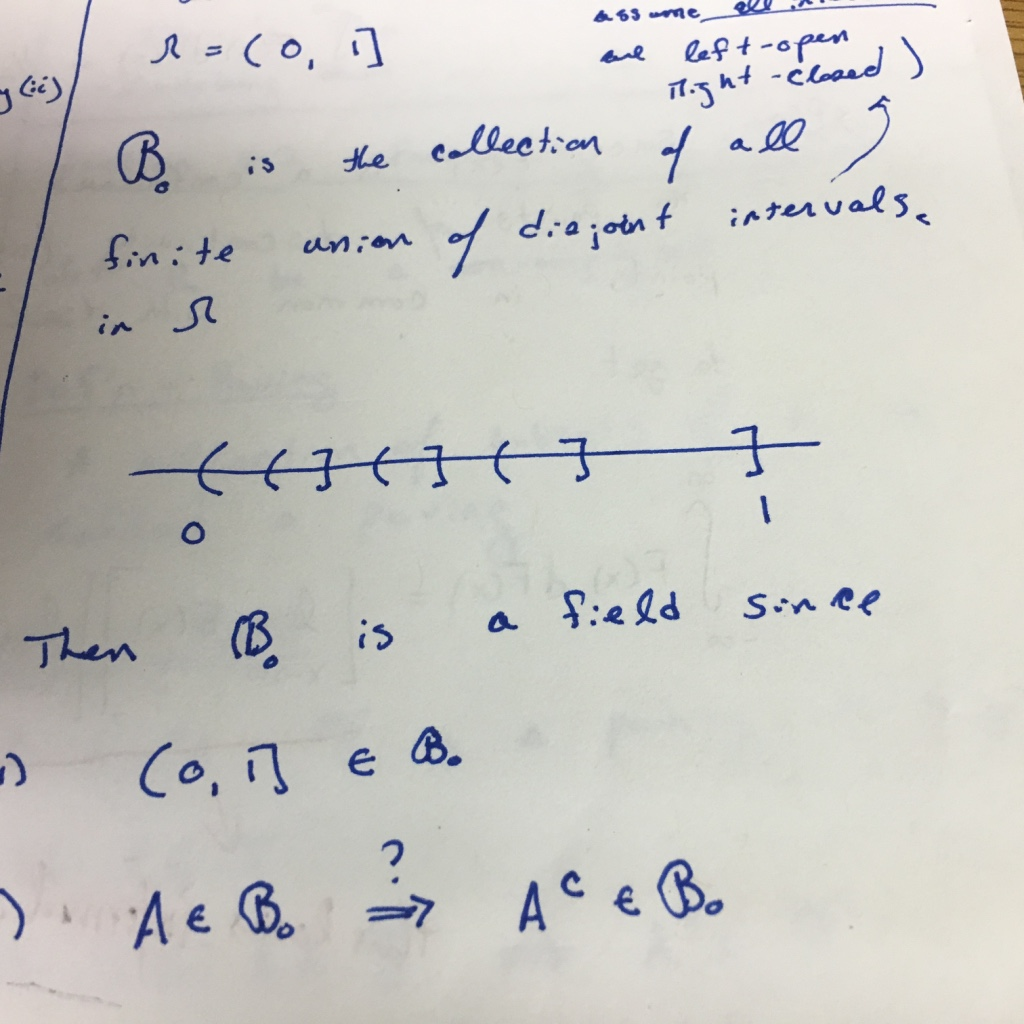
\includegraphics[scale=0.15]{notes1.jpg}
	\caption{Finite unioin of three disjoint intervals.}
	\end{figure}

	Then $\mathcal{B}_0$ is a field. 

	\begin{enumerate}[label = (\roman*)]
		\item (0, 1] $\in \mathcal{B}_0$
		\item $A \in \mathcal{B}_0 \Rightarrow A^c \in \mathcal{B}_0$ 
		\begin{figure}[h]
		\centering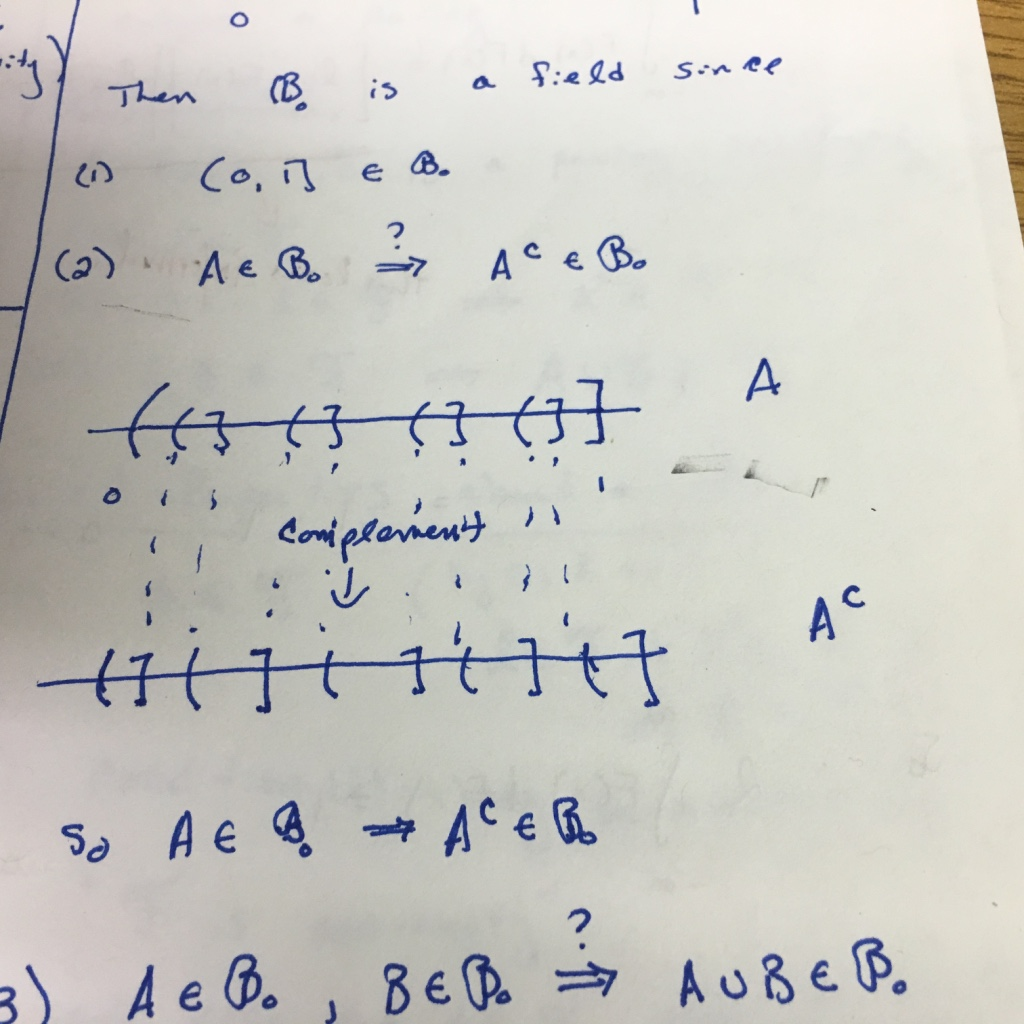
\includegraphics[scale=0.15]{notes2.jpg}
		\caption{A and complement of A.}
		\end{figure}

		\item $A \in \mathcal{B}_o, B \in \mathcal{B}_o \Rightarrow A \bigcup B \in \mathcal{B}_o$ 

		\begin{figure}[h]
		\centering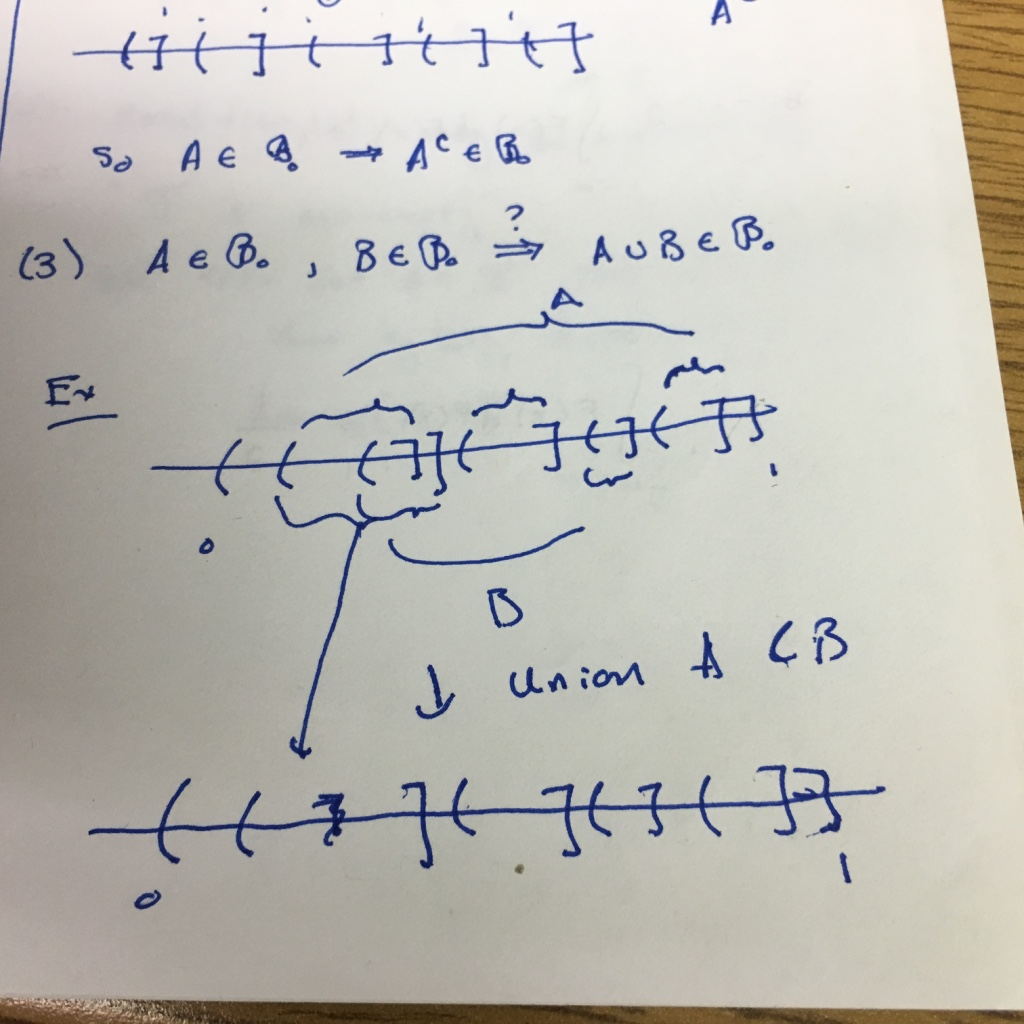
\includegraphics[scale=0.15]{notes3.jpg}
		\caption{Union of A and B is still in $\mathcal{B}_o$}
		\end{figure}

	\end{enumerate}


\end{example}


\textbf{Wednesday August 24}

$\mathcal{B}_0 = $ collection of finite unions of disjoin subintervals of (0, 1]. Is a field. \\
\\

\begin{definition}[Power Set]
	A $\sigma$-field is generated by a paving of power set. Let $\Omega$ be a set. The collection of all subsets of $\Omega$ is the power set written as $2^\Omega$.
\end{definition}

\begin{remark}
	Where does this notation come from?

Consider ths case where $\Omega$ is finite

$$\Omega = \{\omega_1, \dots, \omega_n \} $$

Total number of subsets of $\Omega$. 

$\emptyset, 1$ element sets, 2-element sets, $\dots$, n-element ests.

$$() + () + \dots + = (1+1)^n$$

$\#(\mathcal{F})  = 2^{\# \Omega}$, so it seems reasonable to denote $\mathcal{F} = 2^\Omega$. 

It is also easy to show that $2^\Omega$ is a $\sigma$-field. (The largest, even. The smallest: $\{\emptyset, \Omega\}$ which is also a $\sigma$-field.)

$$\{\emptyset, \Omega\} \subseteq \sigma\text{-field} \subseteq 2^\Omega$$ 
\end{remark}

It turns out we can extend notion of lenght from $\mathcal{B}_0$ to $\sigma$-field generated by $\mathcal{B}_o$. \\
\\
Now, let $\mathcal{A}$ be a nonempty paving of $\Omega$. We define 
$$\sigma(\mathcal{A}) = \bigcap \{\mathcal{B} \subseteq 2^\Omega: \mathcal{B}\text{ is a }\sigma\text{-field}, \mathcal{A} \subseteq \mathcal{B}\} $$

OR rather, the \textit{intersection} of all $\sigma$-fields that contains $\mathcal{A}$. \\
\\
Let 
$$\mathbb{F}(\mathcal{A}) = \{\mathcal{B} \subseteq 2^\Omega: \mathcal{B} \text{ is a } \sigma\text{-field, } \mathcal{B} \supseteq \mathcal{A} \}$$

Then, 
$$\sigma(\mathcal{A}) = \bigcap \mathcal{B}$$
$$\mathcal{B} \in \mathbb{F}(\mathcal{A}) $$

\textbf{Derived Facts}

$\mathbb{F}(\mathcal{A})$ is nonempty. For example, $2^\Omega$ is a $\sigma$-field and $2^\Omega \supseteq \mathcal{A}$. 

$\bigcap  B$ is a $\sigma$-field. ($B \in \mathbb{F}(\mathcal{A})$)

\begin{remark}
	Get notes about notation/levels.
\end{remark}

\begin{proof} We will prove that indeed $\sigma(\mathcal{A})$ is a $\sigma$ -field. Recall that we have three conditions above for $\sigma$-field.\\
\\
	\begin{enumerate}[label = (\roman*)]
		\item $$\Omega \in \sigma(\mathcal{A})$$ 
			$$\Omega \in \cap_{B \in \mathbb{F}(\mathcal{A})} B $$
			Because: B is $\sigma$-field, $A \in B$, $\forall B \in \mathbb{F}(\mathcal{A})$.
		\item 
			$\begin{aligned}
							A \in \bigcap  B &\Rightarrow A \in B \forall B \in\mathbb{F}(\mathcal{A})\\
							&\Rightarrow A^C \in B , \forall B  \in \mathbb{F}(\mathcal{A})\\ 
							&\Rightarrow A^C \in \cap_{B \in \mathbb{F}}(\mathcal{A}) B\\
						\end{aligned}$

		\item $A_1, \dots, \in \cap_{B \in \mathbb{F}(\mathcal{A})} B, \forall  B  \in \mathbb{F}(\mathcal{A})$

		$\Rightarrow \bigcup^\infty_{n =1} A_n \in B, \forall B \in \mathbb{F}(\mathcal{A})$

	\end{enumerate}

	So, $\sigma(\mathcal{A}$ is a $\sigma$-field, we call it the $\sigma$-field, generated by $\mathcal{B}_o$. We know how tot assign lenth to members of $\mathcal{B}_o$, we now show the assignment can be extended to $\sigma(\mathcal{B}_o)$ 


\end{proof}

\begin{example}
	 Let $\mathcal{I}$ be the collection of \textit{all} subintervals of (0,1].\\
	\\
	 Note that $\mathcal{I}$ is a smaller collection than $\mathcal{B}_0$ since $\mathcal{B}_0$ can have numerous different combinations of the sets. 

	 Let

	$$\mathcal{B} = \sigma(\mathcal{I})$$. 

	This is a Borel-$\sigma$-field. (a member of $\mathcal{B}$ in Borel set.)

	It turns out

	$$\sigma(\mathcal{I}) = \sigma(\mathcal{B}_o)  $$

This is because $\sigma(\mathcal{I})$ is a $\sigma$-field. 

So, 
	\begin{align*}
		\sigma(\mathcal{I}) &\supseteq \mathcal{B}_o\\
		\sigma(\mathcal{I}) &\supseteq \sigma(\mathcal{B}_o)
	\end{align*}

Also, 
\begin{align*}
		\mathcal{I} &\subseteq \mathcal{B}_o\\
		\sigma(\mathcal{I}) &\subseteq \sigma(\mathcal{B}_o)
	\end{align*} 

Thus, 
\begin{align*}
	\sigma(\mathcal{I}) &= \sigma(\mathcal{B}_o)
\end{align*}
\end{example}




\begin{definition}[Probability Measure]

Probablity measures on field. Suppose $\mathcal{F}$ is a field on a nonempy set $\Omega$. A probability measure is a function $P:\mathcal{F} \rightarrow \mathbb{R}$. 

\begin{enumerate}[label = (\roman*)]
	\item $0 \leq P(A) \leq 1, \forall A \in \mathcal{F}$
	\item $P(\emptyset) = 0$, $P(\Omega) = 1$
	\item If $A_1, \dots$ are disjoint emembers of $\mathcal{F}$ and $\bigcup A_n \in \mathcal{F}$ then we have countable additivity:

	$$P (\bigcup A_n) = \displaystyle\sum^\infty_{n=1} P(A_N) $$
\end{enumerate}

\begin{remark}
	Note that (iii) also implies finite additivity. Prove by adding infinite empty sets on end. 
\end{remark}

	
\end{definition}


If $\Omega$ is nonempty set. 
And $\mathcal{F}$ is a $\sigma$-field on $\Omega$.
And P is a probability measure on $\mathcal{F}$.

Then ($\Omega, \mathcal{F}, P$) is called a \textbf{probability space.}

And ($\Omega, \mathcal{F}$) is called a \textbf{measurable space.}


\begin{remark}
	If $A \subseteq B$, then $P(A) \leq P(B)$. This is because we may write B as

	$$B = A \bigcup (B\setminus A) $$
\end{remark}

\begin{remark}
	$$P(A) + P(B) = P(A\bigcup B) + P(A \bigcap  B)$$


\end{remark}

\textbf{Friday August 26}
\\

Recall, 

Probability measure on a field, $\mathcal{F}_0$.

\begin{itemize}
	\item $P(A) + P(B) = P(A\bigcup B) + P(A \bigcap  B)$

	% GET VINN DIAGRAM
	\begin{itemize}
		\item $P(A) = P(AB^C) + P(A B)$
		\item $P(B) = P(B A^C) + P(AB)$
		\item $P(A) + P(B) = P(AB^C) + P(BA^C) + 2P(AB)$
		\item $P(A \bigcup B) = P(AB^C) + P(BA^C) + P(AB)$ 
	\end{itemize}
	
	\item $P(A \bigcup B) = P(A) + P(B) - P(AB)$
		By induction, we can prove if $A_1, \dots A_n$,

		$$P(\displaystyle \bigcup^n_{k=1} A_k) = \displaystyle \sum^n_{k=1} P(A_k) - \displaystyle \sum_{i<j} P(A_iA_j) +
		\displaystyle \sum_{i<j<k} A_iA_j) + \dots + (-1)^{n+1} P(A_1, \dots, A_n)  $$

		Inclusion- Exclusion Formula

	\item If $A_1, \dots A_n \in \mathcal{F}$,

		$$B_1 = A_1 $$
		$$B_2 = A_2 \setminus A_1$$
		$$\vdots $$

		Then, 
		$$\displaystyle \bigcup^n_{k=1} A_k = \displaystyle \bigcup^n_{k=1} B_k $$

		but the $B_i$ are disjoint. Also $A_K \subseteq B_k \forall k=1, \dots, n$.

		$$ P(\displaystyle \bigcup^n_{k=1} A_k) = P(\displaystyle \bigcup^n_{k=1} B_k) = \displaystyle \sum^n_{k=1} B_k \leq \displaystyle \sum^n_{k=1} A_k$$

		Thus, $P(\displaystyle \bigcup^n_{k=1} A_k) \leq \displaystyle \sum^n_{k=1} A_k$. Finite subadditivity. 

\end{itemize}

Some conventions, 

If $A_1, \dots$ is a sequence of sets, we say $A_n \uparrow A$ if 

\begin{enumerate}
 	\item $A_1 \subseteq A_2 \subseteq \dots$
 	\item $\displaystyle \bigcup^\infty_{k=1} A_k = A$
 \end{enumerate} 
\vspace{5mm}
 If $A_1, \dots$ is a sequence of sets, we say $A_n \downarrow A$ if 

\begin{enumerate}
 	\item $A_1 \supseteq A_2 \supseteq \dots$
 	\item $\displaystyle \cap^\infty_{k=1} A_k = A$
 \end{enumerate} 

 \begin{theorem}
 	If $P$ is a probability measure on a field $\mathcal{F}$ Then, 

 	\begin{enumerate}
 		\item Continuity from below.

 		If $A_n \in \mathcal{F} \quad \forall n, A \in \mathcal{F}$
 		$$ A_n \uparrow A$$

 		then $$P(A_n) \uparrow P(A)$$

 		\item Continuity from above.

 		If $A_n \in \mathcal{F} \quad \forall n. A \in \mathcal{F}$  
 			$$A_n \downarrow A$$
 		 then $$P(A_n) \downarrow P(A)$$

 		\item Countable subadditivity.

 		If $A_n \in \mathcal{F} \quad \forall n. \displaystyle \bigcup^\infty_{k=1} A_k \in \mathcal{F}$ then 

 		$$P(\displaystyle \bigcup^\infty_{n=1} A_k) \leq \displaystyle \sum^\infty_{n=1} P(A_k)$$
 	\end{enumerate}
 \end{theorem}

 \begin{proof}

 \begin{enumerate}
 	\item If $A_1, \dots A_n \in \mathcal{F}$,

		$$B_1 = A_1 $$
		$$B_2 = A_2 \setminus A_1$$
		$$B_3 = A_3 \setminus A_2$$
		$$\vdots $$

		then, $B_1, \dots$ are disjoint. 

		$$\displaystyle \bigcup^\infty_{n=1} A_n = \displaystyle \bigcup^\infty_{n=1} B_n $$

		$\begin{aligned}
			P(A) &= P(\displaystyle \bigcup^\infty_{n=1} A_n) \\
		&= P(\displaystyle \bigcup^\infty_{n=1} B_n ) \\
		&= \displaystyle \sum^\infty_{n=1} P(B_n) \\
		&= \lim_{n \rightarrow \infty} \displaystyle \sum^\infty_{n=1} P(B_n)\\ 
		&= \lim_{n \rightarrow \infty} P(A_n)
		\end{aligned}
		$

	\item $A_n \downarrow A \Leftrightarrow A_n^C \uparrow A^C$

	But by (1), 

	$$P(A_n^C) \uparrow P(A^C)$$
	$$1 - P(A_n) \uparrow 1 - P(A)$$
	$$P(A_n) \downarrow P(A)$$


	\item By finite subadditivity, 

	$$ P(\displaystyle \bigcup^n{k=1} A_k) \leq \displaystyle \sum^n{k=1} P(A_k) \leq \displaystyle \sum^\infty_{n=1} P(A_n)$$

	But since, by (1), because

	$$\displaystyle \bigcup^n_{k=1} A_k \uparrow \displaystyle \bigcup^\infty_{n=1} A_n$$

	$$P(\displaystyle \bigcup^n_{k=1} A_k) \uparrow P(\displaystyle \bigcup^\infty_{n=1} A_n)$$

	So, 

	$$P(\displaystyle \bigcup^\infty_{n=1} A_n) \leq
		 \displaystyle \sum^\infty_{n=1} P(A_n)$$


 \end{enumerate}
\end{proof}

\begin{remark}
	$A \in \mathcal{F} =$ "A is F-set".
\end{remark}


\section{Extention of Probability Measure to a $\sigma$-field}\index{Exten. Prob Measure to $\sigma$-field}

Let $f$ be a function $f: D\rightarrow R$. 

Let $\tilde{D}$ be another set such that 

$$D \subseteq \tilde{D} $$

An extantion of $f$ onto  $\tilde{D}$ is 

$$\tilde{f}: \tilde{D} \rightarrow R $$

Such that $f(x) = \tilde{f}(x) \forall x \in D$

$\tilde{f}$ is an extention of $f$ on D. 

We say $f$ has unique extention, $\tilde{f}$ onto $\tilde{D}$ if 

\begin{enumerate}
	\item $\tilde{f}$ is an extension of $f$ to $\tilde{D}$.

	\item if $g$ is another extension of $f$ to $\tilde{D}$ then $\tilde{f} = g$ on $D$.
\end{enumerate}


\begin{theorem}
	A probability measure on a field has a unique extension on the $\sigma$-field generated by this field. 

		This means that if $\mathcal{F}_0$ is a field, and $P$ is a probability measure on $\mathcal{F}_0$, then there exists a probability measure, $Q$ on $\sigma(\mathcal{F})$ such that 
		$$Q(A) = P(A)\quad \forall A \in \mathcal{F}_0$$

		Moreover, if $\tilde{Q}$ is another probability measure on $\sigma(\mathcal{F}_0)$ such that $\tilde{Q} = P(A) \quad \forall A \in \mathcal{F}$ then $$\tilde{Q} = Q$$. 
\end{theorem}

	\begin{remark}
		The proof of this theorem will come after several definitions and lemmas. 
	\end{remark}

	\textbf{Outer Measure} $P^*: 2^\Omega \rightarrow \mathbb{R}$  

	For any $A \in 2^\Omega$ ($A \subseteq \Omega$)

	$$P^*(A) = \inf \{\displaystyle \sum_{n=1}^\infty P(A_n): A_1, A_2, \dots \text{is a sequence of } \mathcal{F}_0 \text{ sets, } A \subseteq \bigcup^\infty_{n=1} A_n\} $$

	$P^*$ is a measure out until $\mathcal{M}$, but it is only a function beyond that on $2^\Omega$.\\

\textbf{Inner Measure}

$P_*(A) = 1 - P^*(A)$ 

\vspace{5mm}

Define the paving $\mathcal{M}$ as followes
$$\mathcal{M} = \{ A \in 2^\Omega:
		E \in 2^\Omega,
		P^*(E) = P^*(E\bigcap A) + P^*(E \bigcap A^C) \}$$

	Idea: we came up with this $\mathcal{M}$ such that $P^*$ behaves as a measure. It will turn out to be that $\mathcal{M}$ is a $\sigma$-field that contains $\sigma(\mathcal{F}_0)$.\\

\textbf{Monday August 29}\\

$P^*$ satisfies the following probabilities:

\begin{enumerate}[label = (\roman*)]
	\item $P^*(\emptyset) = 0$
	\item $P^*(A) \geq 0 \quad \forall A \in 2^\Omega$
	\item $A \subseteq B \Rightarrow P^*(A) \subseteq P^*(B)$
	\item $P^*(\bigcup^\infty_{n=1} A_n) \leq \displaystyle \sum^\infty_{n=1} P^*(A_n))$
\end{enumerate}

\begin{proof}
	
	\begin{enumerate}[label = (\roman*)]
		\item Take $\{\emptyset, \emptyset, \dots \}$. 

		$$\emptyset \in \mathcal{F}_0, \quad \emptyset \bigcup^\infty_{n=1} \emptyset $$

		So, \\
		$$P^*(\emptyset) \leq \displaystyle \sum^\infty_{n=1} P(\emptyset) = 0$$

		Note,

		$$P(A) \geq 0 \quad \forall A$$

		So, 

		$$P^*(\emptyset) \geq \emptyset$$ 

		Thus,

		 $$P^*(\emptyset) = \emptyset$$
		\item  Already done as part of (i).

		\item  Let $A \subseteq B$

		$$P^*(A) = \inf\{\displaystyle \sum^\infty_{n=1} P(A_n), A_n \in \mathcal{F}_0, A \subseteq \bigcup A_n \} $$

		Now, if $B_1, \dots \in \mathcal{F}_0 \subseteq \bigcup B_n$

		Then, 
		$$A \subseteq B \subseteq \bigcup_n B_n $$

		If  $\{ \{B_n\}^\infty_{n=1}: B_n \in \mathcal{F}_0, B \subseteq \bigcup_n B_n \} \subseteq \{ \{A_n\}^\infty_{n=1}: A_n \in \mathcal{F}_0, A \subseteq \bigcup_n A_n \}$

		Or in short, Collection 1 $\subseteq$ Collection 2.\\

		So the inf of a larger set is smaller than (or equal to) the inf of a smaller set.\\
		
		So, 

		$P^*(A) = \inf\{\displaystyle \sum^\infty_{n=1} P(A_n), A_n \in  \text{ collection \#1}\} \leq P^*(B) = \inf\{\displaystyle \sum^\infty_{n=1} P(B_n), A_n \in  \text{ collection \#2}\} = P^*(B)$

		\item Want 

		$$P^*(\bigcup_n A_n) \leq \displaystyle\sum_n P^*(A_n) $$

		$P^*(A_n) = \inf \{\displaystyle \sum_{n=1}^\infty P(A_n): A_{nk} \in \mathcal{F}_0,  A \subseteq \bigcup_{k} A_{nk}\}$\\

		Let $\epsilon > 0$, by defnition of  there exists, 

		$$ \{B_n\}^\infty_{n=1}  $$ such that

		$$\displaystyle \sum^\infty_{k=1} P(B_{nk}) \leq P^*(A_n) + \frac{\epsilon}{2^n} $$

		So, 

		$$\bigcup_n A_n \subseteq \bigcup_{n,k} B_{nk} $$

		and,\\

		$\begin{aligned}
			P^*(\bigcup_n A_n) &\leq \displaystyle \sum_{n,k} P(B_{nk})\\ 
			&< \displaystyle \sum_n P^* (A_n) + \sum_n (\epsilon 2^{-n})\\
			P^*(\bigcup A_n) &< \sum_n P^* (A_n) + \epsilon \quad \forall \epsilon > 0
		\end{aligned}$

		Simply put, \\
		$ b$

		So, 

		$$P^*(\bigcup_n A_n) \leq \sum_n P^*(A_n) $$
 	\end{enumerate}
\end{proof}

By definition, $A \in \mathcal{M}$ if and only if $P^*(EA) + P^*(EA^C) = P^*(E)$. \\

We know that $P^*$ is subadditive. \\

So, by subadditivity we know, 

$$P^*(E) \leq P^*(AE) + P^*(A^C E) $$

Therefore, to show $A \in \mathcal{M}$ we only need to show 

$$P^*(E) \geq P^*(AE) + P^*(A^C E) $$


$\mathcal{M}$ is defined by $P^*$ and $P^*$ is defined using $\mathcal{F}_0$ so $\mathcal{M}$ is indireclty tied to $\mathcal{F}_0$.\\

\textbf{Lemma 1.} $\mathcal{M}$ is a field.

\begin{proof}


\begin{enumerate}[label = (\roman*)]
	\item $\Omega \in \mathcal{M}$\\

	$$\begin{aligned}
			A &= \Omega\\
			P^*(\emptyset) &= 0\\
			P^*(E) + P^*(\emptyset) &= P^*(E)
		\end{aligned}$$

	\item $A \in \mathcal{M} = A^C \in \mathcal{M}$\\

	$$\begin{aligned}
		P^*(E) &= P^*(EA) + P^*(A^C E)\\
		&= P^*(EA^C) + P^*(A E)\\
		&= P^*(EA^C) + P^*((A^C)^C E)
	\end{aligned}$$

	\item $A, B \in \mathcal{M} \rightarrow A \bigcap B \in \mathcal{M}$\\

	$B \in \mathcal{M} \Rightarrow P^*(E) = P^*(Eb) + P^*(B^C E) \quad \forall E$

	$A \in \mathcal{M} \Rightarrow P^*(BE) = P^*((BE)A) + P^*(A^C (BE))$

	$A \in \mathcal{M} \Rightarrow P^*(B^CE) = P^*((B^CE)A) + P^*(A^C (B^CE))$\\

	Hence, \\
	
	$$P^*(BE) + P^*(B^CE) = P^*((BE)A) + P^*(A^C (BE)) + P^*((B^CE)A) + P^*(A^C (B^CE))$$

	$$\begin{aligned}
		P^*(A^C (BE)) + P^*((B^CE)A) + P^*(A^C (B^CE)) &\geq P^*((A^C BE) \bigcup (AB^CE)\bigcup(A^CBE))\\
			&= P^*(E\cap[A^CB\bigcup  AB^C\bigcup A^CB^C])\\
			&= P^*(E \bigcap (AB)^C)
	\end{aligned} $$

	$$\begin{aligned}
		P^*(E) &= P^*(BE) + P^*(B^CE)\\
		&= P^*((BE)A) + (P^*(A^C (BE)) + P^*((B^CE)A) + P^*(A^C (B^CE)))\\
		&\geq P^*(ABE) + P^*(E(AB)^C)
	\end{aligned} $$
	
	 

	So, $A,B \in \mathcal{M}$
\end{enumerate}
\end{proof}

\textbf{Lemma 2.} If $A_1, A_2, \dots$ is a sequence of disjoint $\mathcal{M}$-sets then for each $E \subseteq \Omega$, 
$$P^*(E\cap(\bigcup_k A_k)) = \displaystyle \sum_k P^*(E \bigcap A_k) $$

\begin{proof}
	First, prove this statement for finite sequence. 

	$$A_1, \dots, A_n $$

	by mathematical induction. \\
	\\

	If $n=1$ this is 'trivial', 

	$$P^*(E\bigcap A_1) = P^*(E \bigcap A_1) $$

	If $n = 2$ we need to show, 

	$$ P^*(E  (A_1 \bigcup A_n)) = P^*(E A_1) + P^*(E A_2)$$

	Because $A_1 \in \mathcal{M}$, 

	$$P^*(E(A_1 \bigcup A_2)) = P^*(E(A_1 \bigcup A_2)) A_1 + P^*(E(A_1 \bigcup A_2)A_1^2)  $$

	$$E(A_1 \bigcup A_2) = E(A_1 A_2 \bigcup A_1 A_2 = EA_1$$

	$$E(A_1 \bigcup A_2) A_1^C = E(A_1 A_1^C \bigcup A_2 A_2^C)$$

	So, 

	$$P^*(E(A_1 \bigcup A_2)) = P^*(EA_1) + P^*(EA_2)$$

Suppose true for n = k. (induction hypothesis) \\
\\
Now we must show for n = k + 1.

$$P^* (E \bigcap (\bigcup_{n=1}^{k+1} A_n)) = P^*([E \bigcap (\bigcup_{n=1}^{k} A_n)] \bigcup A_{k+1}) $$

$ (\bigcup_{n=1}^{k} A_n), A_{k+1}$ are two disjoint sets. Using the n=2 case, 

$$ = \displaystyle \sum_{n=1}^k P^*(E \bigcap A_n) + P(E \bigcap A_{k+1}) = \displaystyle \sum_{n=1}^{k+1} P^*(E \bigcap A_n)  $$

So this is now shown to be true for $\{A_1, \dots, A_n \}$. Next, showtrue for $A_1, \dots in \mathcal{M}$ (disjoint).

Want: 

$$P^*(E \bigcap (\bigcup_{n=1}^\infty A_n)) = \displaystyle \sum_{n=1}^{\infty} P^*(E \bigcap A_n)  $$

Using countable subadditivity, 

$$ P^*(E \bigcap (\bigcup_{n=1}^\infty A_n)) = P^*(\displaystyle \bigcup_{n=1}^{\infty} E \bigcap A_n) \leq \displaystyle \sum_{n=1}^{\infty} P^*(E \bigcap A_n)$$

In the meantime, by the monotonicity of $P^*$

$$P^*(E \bigcap (\bigcup_{n=1}^\infty A_n)) \geq P^*(E \bigcap (\bigcup_{n=1}^m A_n)) =  \displaystyle \sum_{n=1}^{\infty} P^*(E \bigcap A_n)$$

So, 

$$P^*(E \bigcap (\bigcup_{n=1}^\infty A_n)) \geq \lim  \displaystyle \sum_{n=1}^{m} P^*(E \bigcap A_n)$$


(*), (**) gives us, 

$$P^*(E \bigcap (\bigcup_{n=1}^\infty A_n)) = \displaystyle \sum_{n=1}^{\infty} P^*(E \bigcap A_n)  $$

\end{proof}

\textbf{Wednesday August 31}

(finished proof)\\
\\

\textbf{Lemma 3.}
	
	\begin{enumerate}
		\item $\mathcal{M}$ is a $\sigma$-field
		\item $P^*$ restricted on $\mathcal{M}$ is countably additive. 
	\end{enumerate}

\begin{proof}
	First we show if\\

	\begin{enumerate}
		\item $\mathcal{M}$ is a fieldd
		\item $\mathcal{M}$ is closed under countable disjoint union.
	\end{enumerate}

then $\mathcal{M}$ is a $\sigma$-field.

Let's create disjoints sets, 

$A_n \in \mathcal{M}, n = 1, 2, \dots$
$B_1 = A_1$
$B_2 = A_2 A^C_1$
$\vdots$
$B_n = A_n A_1^C \dots A_{n-1}^C$

$B_1, \dots, B_n \in \mathcal{M}$ (disjoint)


$$\bigcup^\infty_{n=1} B_n = \bigcup^\infty_{n=1} A_n $$

But we know that $\bigcup^\infty_{n=1} B_n \in \mathcal{M}$ so $\bigcup^\infty_{n=1} A_n \in \mathcal{M}$ and thus $\mathcal{M}$ is a $\sigma$-field.

So it suffices to show that $\mathcal{M}$ is closed under disjoint countable unions.\\
\\
Let $A_1, A_2, \dots$ are disjoins $\mathcal{M}$-sets.\\ 
\\
Let $A = \bigcup^\infty_{n=1} A_n$.\\ 
\\
Let $F_n = \bigcup^n{k=1} A_k$.\\ 
\\
Then $F_n \in \mathcal{M}$.\\
\\
So, $\forall E \in 2^\Omega$, 

$$P^*(E) = P^*(E F_n) + P^*(E F_n^C) $$

\begin{align*}
	P^*(E F_n) &= P^*(E(\bigcup_{k=1}^n A_k))\\
		&= \displaystyle \sum^n_{k=1} P^*(E A_k)\\
P^*(E F_n^C) &\geq P^*(E A^C)  (F_n \subseteq A, F_n^C \supseteq A^C)\\
	\Rightarrow P^*(E) \geq \lim_{n \rightarrow \infty} P^*(E A_k) + P^*(E A^C)\\
		&= \displaystyle \sum^n_{k=1} P^*(E A_k) + P^*(E A^C)\\
		&= P^*(EA) + P^*(E A^C)
\end{align*}
 

\end{proof}

So $A \in \mathcal{M}$ and $\mathcal{M}$ is a $\sigma$-field. \\
\\

Now, let's show $P^*$ is countably additive.

Let $A_1, A_2, \dots$ be disjoint members of $\mathcal{M}$. Then $\forall E \in 2^\Omega$, 

$$P^*(E(\bigcup^\infty_{n=1} A_n)) = \displaystyle \sum^\infty_{n=1} P(E A_n) $$

Take $E = \Omega$. 

$$P^*(\bigcup^\infty_{n=1} A_n) = \displaystyle \sum^\infty_{n=1} P( A_n) $$


\textbf{Lemma 4.} $\mathcal{F}_0 \subseteq \mathcal{M}$

\begin{proof}
	Let $A \in \mathcal{F}$.\\
	\\

	Want:

	$$A \in \mathcal{M} $$
$$P^*(E) = P^*(EA) + P^*(E A^C) $$

By definition, there exists $E_n \in \mathcal{F}_0$ 
such that 

$$\displaystyle \sum^\infty_{n=1} P^*(E_n) \leq P^*(E) + \epsilon $$

$\begin{aligned}
	P^*(EA) &\leq P^*((\bigcup^\infty_{n=1} E_n)A) \text{ (monotonocity)}\\
		&= P^* (\bigcup^infty_{n=1} (E_n A))\\
		&\leq \displaystyle \sum^infty_{n=1}P^* ( (E_n A)) \text{ (countibly subadd)}\\
	P^*(E A^C) &\leq \displaystyle \sum^\infty_{n=1} P^*(E_n A^C)\\
	P^*(EA) + P^*(E A^C) &\leq 	\displaystyle \sum^\infty_{n=1} P^*(E_n A) + P^*(E_n A^C)\\
		&= \displaystyle \sum^\infty_{n=1} P^*(E_n)\\
	\text{Recall, } A, E_n \in \mathcal{F}_0\\
		&\leq P^*(E) + \epsilon\\
	P^*(EA) + P^*(E A^C) & \leq P^*(E) + \epsilon \quad \forall \epsilon\\
	\Rightarrow P^*(EA) + P^*(EA^C) &= P^*(E)\\
	\Rightarrow A \in \mathcal{M}\\
	\mathcal{F}_0 \in \mathcal{M}
\end{aligned}$
 
\end{proof}

\textbf{Lemma 5.}$$P^*(A) = P(A) \quad \forall A \in \mathcal{F}_0$$

\begin{proof}
	Let $A \in \mathcal{F}_0$. 

	Because,  $A, \emptyset, \emptyset, \dots, \in \mathcal{F}_0$. 

	$$A \subseteq A \bigcup \emptyset \bigcup \emptyset \dots $$

	$$P^*(A) \leq P(A) + P(\emptyset) + \dots $$

But, if 

$$A_n \in \mathcal{F}_0$$

$$A \subseteq \bigcup^\infty_{n=1} A_n $$

$$P^*(A) \leq \displaystyle \sum^\infty_{n=1} P(A_n)$$

$$\Rightarrow P^*(A) \leq \inf \displaystyle \sum^\infty_{n=1} P(A_n) $$

$$ = P^*(A)$$
\end{proof}

\textbf{Friday September 2}

\begin{remark}
	\textbf{5 Lemma Recap}

	\begin{tabular}{|p{0.9\linewidth}|}\hline % or any other width
\rule{0pt}{5ex}% for more vertical space
		
	\textbf{Lemma 1.} $\mathcal{M}$ is a field.

	\textbf{Lemma 2.} If $A_1, A_2, \dots$ is a sequence of disjoint $\mathcal{M}$-sets then for each $E \subseteq \Omega$, 
	$$P^*(E\cap(\bigcup_k A_k)) = \displaystyle \sum_k P^*(E \bigcap A_k) $$

	\textbf{Lemma 3.}
	
	\begin{enumerate}
		\item $\mathcal{M}$ is a $\sigma$-field
		\item $P^*$ restricted on $\mathcal{M}$ is countably additive. 
	\end{enumerate}
	
	\textbf{Lemma 4.} $$\mathcal{F}_0 \subseteq \mathcal{M}$$
	\textbf{Lemma 5.}$$P^*(A) = P(A) \quad \forall A \in \mathcal{F}_0$$
	\text{ }\\
	\\\hline
\end{tabular}
\end{remark}

Recall, Extension Theorem. That is, If $\mathcal{F}$ is a field and $P$ is a probability measure, then there exists a measure, $Q$ such that 

	$$Q(A) =  P(A) \quad \forall A \in \mathcal{F}_0$$

\begin{proof}
	By Lemma 5, \\
\\
	$P^*(\Omega) = P(\Omega) = 1$\\
	$P^*(\emptyset) = P(\emptyset) = 0$\\
	\\

	Outline of what we need to show:\\

	\begin{itemize}
		\item $ 0 \leq M(A) \leq 1$
		\item $M(\emptyset) = 0, \quad M(\Omega)=1$
		\item $M(\bigcup_n A_n) = \sum_n M(A_n)$
	\end{itemize}

	\vspace{5mm}

	Since $\forall A \in \mathcal{M}$, 

	$$\emptyset \subseteq A \subset \Omega $$

	then 

	$$ 0 \leq P^*(\emptyset) \leq P^*(A) \leq P^*(\Omega) \leq 1$$

	But, by Lemma 3, $P^*$ is contably additive on $\mathcal{M}$. So $P^*$ is probability measure on $\mathcal{M}$ (which is a $\sigma$-field, by Lemma 3).\\

	By Lemma 4, $\mathcal{F}_0 \subset \mathcal{M} \Rightarrow \sigma(\mathcal{F}_0 \subseteq \mathcal{M}$. So $P^*$ is also probabliity measure on $\sigma(\mathcal{F}_0).$\\

	Finally, by Lemma 5, again $P^*(A) = P(A)$, $P^*$ is an extention of $P$ form $\mathcal{F}_0$  to $\sigma(\mathcal{F}_0)$. \\
\end{proof}

\textit{Uniqueness of of the extention, $\pi-\lambda$ Theorem}\\

	Paving - $\{ \pi$-system and $\lambda$-system.$\}$ (?)\\

\begin{definition}[$\pi$-System]
	A class of subsets $\mathcal{P}$ of $\Omega$ is a $\pi$ system, if $$A, B \in \mathcal{P} \Rightarrow AB \in \mathcal{P}$$ 
\end{definition}
	
\begin{definition}[$\lambda$-System]
	A class $\mathcal{L}$ is a $\lambda$-system if 
		\begin{enumerate}[label = $\lambda$(\roman*)]
			\item $\Omega \in \mathcal{L}$ 
			\item $A \in \mathcal{L} \Rightarrow A^C \in \mathcal{L}$
			\item If $A_1, \dots \in \mathcal{L} $ are disjoint then $\bigcup^\infty_{n=1} A_n \in \mathcal{L}$
		\end{enumerate}
\end{definition}
	

	So, the only difference is "disjoint". Weaker than a $\sigma$-field (i.e. A $\sigma$-field is always a $\lambda$-system).

Note that $(\lambda_2)$ can be replace by $(\lambda_{2\prime})$ wherein

$$A, B \in \mathcal{F}, A \subseteq B, \Rightarrow B\setminus A \in \mathcal{L} $$

That is $\lambda_1, \lambda_2, \lambda_3 \Leftrightarrow \lambda_1, \lambda_{2\prime}, \lambda_3$\\

\textbf{Lemma 6.} A class of sets that is both $\pi$-systema and $\lambda$-system is a $\sigma$-field. 

\begin{proof}
	Suppose $\mathcal{F}$ is both $\pi$-system and $\lambda$-system.

By definition, 
\begin{enumerate}
			\item $\Omega \in \mathcal{F}$ 
			\item $A \in \mathcal{F} \Rightarrow A^C \in \mathcal{F}$
		\end{enumerate}

		Let $A_1, A_2, \dots$ be $\mathcal{F}$ sets. 

		Let's constructs disjoints sets, B

		\begin{align*}
			B_1 &= A_1\\
			B_2 &= A_1A_2^C\\
			\vdots
		\end{align*}

		Then $B_n$ are $\mathcal{F}$-sets (by $\lambda_{2\prime} - A_2^C = \Omega A)2^C \in \mathcal{F}$, by $\pi$-system, $A_1A_2^C \in \mathcal{F}$ ).\\

		By $\lambda_3$, 

		$$\bigcup_n^\infty B_n \in \mathcal{F} $$

		So, 

		$$\bigcup_n^\infty A_n \in \mathcal{F} $$

\end{proof}

\begin{theorem}[$\pi$-$\lambda$ Theorem]
	If $\mathcal{P}$ is in a $\pi$-system, $\mathcal{L}$ is in a $\lambda$-system, then 
	$$\mathcal{P} \subseteq \mathcal{L} \Rightarrow \sigma(\mathcal{P} \subseteq \mathcal{L}) $$
\end{theorem}

\begin{proof}
	Let $\lambda(\mathcal{P})$ be the intersection of all $\lambda$-system that contains $\mathcal{P}$. 

		$$ \lambda(\mathcal{P}) = \cap\{\mathcal{L}^\prime: \mathcal{L}^\prime \supseteq \mathcal{P}, \mathcal{L}^\prime \text{ is }\lambda\text{-set }\}$$

	$\lambda(\mathcal{P})$ is a $\lambda$-system.\\

	Goal: prove $\lambda(\mathcal{P})$ is a $\sigma$-field.
	So we want to show that $\lambda(\mathcal{P})$ is a $\pi$-system.

	\begin{enumerate}
		\item $\Omega \in \lambda(\mathcal{P})$?\\

			$$\Omega \in \mathcal{L}^\prime \quad \forall \mathcal{L}^\prime$$
			$$\Omega \in \lambda(\mathcal{P}) $$

		\item $A \in \lambda(\mathcal{P}) \Rightarrow A^C \in \lambda(\mathcal{P})$?\\

		$$A \in \lambda(\mathcal{P}) \Rightarrow A \in \cap\{\mathcal{L}^\prime: \mathcal{L}^\prime \supseteq \mathcal{P}, \mathcal{L}^\prime \text{ is }\lambda\text{-set }\} $$

		Then 

		$A \in \mathcal{L}^\prime$ for any $\mathcal{L}^\prime \supseteq \mathcal{P}, \mathcal{L}^\prime$ is $\lambda$-system. 

		$$\Rightarrow A^C \in \mathcal{L}^\prime $$

		$$\Rightarrow A^C \in  \cap\{\mathcal{L}^\prime: \mathcal{L}^\prime \supseteq \mathcal{P}, \mathcal{L}^\prime \text{ is }\lambda\text{-set }\} = \lambda(\mathcal{P})$$

		\item $A_1, A_2, \dots \in \lambda(\mathcal{P})$ are disjoint then $A_1, A_2, \dots \in \mathcal{L}^\prime \quad \forall \mathcal{L}^\prime$. 

		Then $\bigcup A_n \in \mathcal{L}^\prime (\mathcal{L}^\prime \lambda\text{-system})$

		So $\bigcup_n A_n \in \lambda(\mathcal{P})$. 

		We call $\lambda(\mathcal{P})$ the $\lambda$-system generated by $\mathcal{P}$.\\

		If we can say that $\lambda(\mathcal{P})$ is also a $\sigma$-field, then $\sigma(\mathcal{P}) \subseteq \lambda(\mathcal{P})$ because $\sigma(\mathcal{P})$ is smallest. So then, $\sigma(\mathcal{P}) \subseteq \mathcal{L}$ because $\lambda(\mathcal{P})$ is the small $\lambda$-system. 

		So it suffices to show that $\lambda(\mathcal{P})$ is a $\sigma$-field. But we know if $\lambda(\mathcal{P})$ is a system then $\lambda(\mathcal{P})$ is $\sigma$-field. So it suffices to show that $\lambda(\mathcal{P})$ is a $\pi$-system.  \\

		Construct again for any $A \in 2^\Omega \quad (A \subseteq \Omega)$, let

		$$\mathcal{L}_A = \{B: AB \in \lambda(\mathcal{P}) \}$$

		Claim: If $A \in \lambda(\mathcal{P})$ then $\mathcal{L}_A$ is $\lambda$-system.\\

		\begin{enumerate}
			\item $\Omega \in \mathcal{L}_A$? 
				$$A\Omega = A \in \mathcal{L}_A$$
			\item $(\lambda_2^\prime) : B_1, B_2 \in \mathcal{L}_A, B_1 \subseteq  B_2 \Rightarrow B_2B_1^C \in \mathcal{L}_A $?

			$$B_1 \in \mathcal{L}_A \Rightarrow AB_1 \in \lambda(\mathcal{P}) $$
			$$B_2 \in \mathcal{L}_A \Rightarrow AB_2 \in \lambda(\mathcal{P}) $$

			Since $AB_1 \subseteq AB_2$, $\lambda(\mathcal{P})$ is $\lambda$-system by ($\lambda_2^\prime$) for $\lambda(\mathcal{P})$

			% GET FROM PHOTO

			\item If $B_n$ is disjoint, $\mathcal{L}_A$-sets. 

			Want $\bigcup_n B_n$ because 

			$$B_n \in \mathcal{L}_A $$

			$$B_n A \in \lambda(\mathcal{P}) $$

			Because $B_n$ disjoint we know that $B_n A$ is also disjoint.

			Hence, 
			$$\bigcup_n(B_n A) \in \lambda(\mathcal{P})$$


		\end{enumerate}

	Claim: $\lambda(\mathcal{P})$ is $\pi$-sytem.

	\begin{enumerate}
		\item If $A \in \mathcal{P}$, then $\mathcal{P} \subseteq \mathcal{L}_A$

	Suppose $A \in \mathcal{P}$.

	Let $B \in \mathcal{P}$, then $AB \in \mathcal{P}$ ($\pi$-system), and $AB \in \lambda(\mathcal{P}) \Rightarrow B \in \mathcal{L}_A$

		\item If $A \in \mathcal{P}$ then $\lambda(\mathcal{P}) \subset \mathcal{L}_A$.

		\item If $A \in \lambda(\mathcal{P})$, then $\mathcal{P} \in \mathcal{L}_A$

		Suppose, $A \in \lambda(\mathcal{P})$ and let $B \in \mathcal{P}$. 

		By step 2,


			$\begin{aligned}
				A &\in \mathcal{L}_A\\
					&\Rightarrow AB \in \lambda(\mathcal{P})\\
					&\Rightarrow B \in \mathcal{L}_A	
			\end{aligned}$

		\item If $A \in \lambda(\mathcal{P})$, then $\lambda(\mathcal{P}) \subseteq \mathcal{L}_A$. This is because $\lambda(\mathcal{P})$ is the smallest $\lambda$-system, $\mathcal{L}_A$ is $\lambda$-system containing $\mathcal{P}$ (by step 3).\\

		Now show that $\lambda(\mathcal{P})$ is $\pi$-system.\\

		$A, B \in \lambda(\mathcal{P})$ because $A \in \lambda(\mathcal{P})$. We have that $\lambda(\mathcal{P}) \in \mathcal{L}_A$.\\

		So 
		$$B \in \mathcal{L}_A $$ 

		$$BA \in \lambda(\mathcal{P})$$

		Thus $\lambda(\mathcal{P})$ is $\pi$-system.
	\end{enumerate}
	\end{enumerate}
\end{proof}

\textbf{Wednesday September 7}

\begin{theorem}
	Suppose $P_1$ and $P_2$ are probability measures on $\sigma(\mathcal{P})$ where $\mathcal{P}$ is a $\pi$-system. If $P_1$ and $P_2$ agree on $\mathcal{P}$ (that is, $P_1(A) = P_2(A) \quad \forall A \in \mathcal{P}$) then they agree on $\sigma(\mathcal{P})$.
\end{theorem}

\begin{proof}
	Let $$\mathcal{L} = \{A \in \sigma(\mathcal{P}): P_1(A) = P_2 (A) \}$$

	Then $\mathcal{P} \subseteq \mathcal{L}$.\\

	It suffices to show that $\mathcal{L}$ is a $\lambda$-system (because if so, then $\sigma(\mathcal{P}) \subseteq \mathcal{L}$ - in fact, $\sigma(\mathcal{P}) = \mathcal{L}$). \\

	Show $\mathcal{L}$ is a $\lambda$-system.\\

	\begin{enumerate}
		\item $\Omega \in \mathcal{L}$?
			$$P_1(\Omega) = P_2(\Omega) = 1, \quad \Omega \in \mathcal{P}$$

		\item $A \in \mathcal{L}$

		$$ P_1(A) = P_2(A) \Rightarrow P_1(A^C) = P_2(A^C), \quad A^C \in \mathcal{L}$$

		\item $A \in \mathcal{L}$. $A_n$ disjoint. Want $\bigcup^\infty_{n=1} A_n \in \mathcal{L}$.

		Since

		$$A_n \in \mathcal{L} $$

		$$P_1(A_n) = P_2(A_n) \quad \forall n$$

		$$\displaystyle \sum^\infty_{n=1} P_1(A_n) = \displaystyle \sum^\infty_{n=1} P_2(A_n) $$

		$$P_1 \displaystyle \bigcup^\infty_{n=1} (A_n) = P_2 \displaystyle \bigcup^\infty_{n=1} (A_n) $$

		So, $\bigcup A_n \in \mathcal{L}$.


	\end{enumerate}
\end{proof}

So our extention of (and uniqueness of the extention of) $P$ on $\mathcal{F}_0$ to $\sigma(\mathcal{F}_0)$ is complete. We have shown the existance of $Q$ on $\mathcal{M}$. \\

Since $Q$ agrees with $P$ on $\mathcal{F}_0$ and $\mathcal{F}_0$ is a field, this implies that this is a $\pi$-system.

If you have another extention, say $\tilde{Q}$, then $\tilde{Q} = P$ on $\mathcal{F}_0$. That is, $\tilde{Q} = Q$ on $\mathcal{M}$, where $\mathcal{M}$ is a $\sigma$-field, which is a $\pi$
-system.\\

So by Theorem 1.3.3, 

$\tilde{Q} = Q$ on $\sigma(\mathcal{P})$. \\

So, Theorem 1.3.1, is completely proved. \\


Lemma 1 - Lemma 5 imply the extention.\\
$\pi-\lambda$ Theorem and Theorem 1.3.3 implies uniqueness. \\
This wraps up Theorem 1.3.1.\\



\textbf{Lebesque measure on (0,1]}

$$\Omega = (0,1]$$

Recall, $\mathcal{B}_0$ is the finite disjoint unions of intervals in (0,1] and that $\mathcal{B}_0$ is a field. \\

Let $\mathcal{B} = \sigma(\mathcal{B}_0)$.\\

For each $A \in \mathcal{B}_0$, 

$$A = \bigcup^n_{i=1} (a_i, b_i] $$

Let $\lambda(A) = \displaystyle \sum^n_{i=1} (b_i - a_i)$.\\

Question: Is $\lambda$ a probability measure on $\mathcal{B}_0$?

\begin{theorem}[Theorem 2.2 in Billingsly]

The set function $\lambda$ on $\mathcal{B}_0$ is a probability measure on $\mathcal{B}_0$.
	
\end{theorem}

\begin{proof}
	\begin{enumerate}
		\item $0 \leq \lambda(A) \leq 1$

		\item $$\lambda(\Omega) = \lambda((0,1]) = 1-0 = 1$$
		$$\lambda(\emptyset) = \lambda((0,0]) = 0$$


		\item This one requires Theorem 1.3 in Billingsly (proof omitted - calculus, blah).

		Theorem 1.3 - If I is an interval in (0,1] and $\{I_k: k=1, 2, \dots \}$ are disjoint intervas in (0,1] such that 

		$$I = \bigcup^\infty_{k=1} I_k$$

		then, 

		$$|I| = \displaystyle \sum^\infty_{k=1} |I_k| $$

		where |a| means length of interval a. 

		Since $\bigcup^{m_k}_{j=1} I_{kj} \in \mathcal{B}_0$ and $\bigcup^{m}_{i=1} I_{i} = \bigcup^\infty_{k=1}\bigcup^{m_k}_{j=1} I_{kj}$.\\

		Then 

		$$\lambda(A) \lambda(\bigcup^{m}_{i=1} I_{i}) = \displaystyle \sum^m_{i=1} |I_i| $$

		Since, $I_i \subset \bigcup^\infty_{k=1}\bigcup^{m_k}_{j=1} I_{kj}$, then 

		$$I_i = I_i(\bigcup^\infty_{k=1}\bigcup^{m_k}_{j=1} I_{kj}) = \bigcup^\infty_{k=1}\bigcup^{m_k}_{j=1} I_i I_{kj} $$

		By Theorem 1.3, 

		$$|I| = \displaystyle \sum^\infty_{k=1} \sum^{m_k}_{j=1} |I_i I_{jk}| $$

		$$\lambda(A) = \displaystyle \sum^m_{i=1} \sum^\infty_{k=1} \sum^{m_k}_{j=1} |I_i I_{jk}| = \displaystyle  \sum^\infty_{k=1} \sum^{m_k}_{j=1} \sum^m_{i=1}|I_i I_{jk}| $$

		Because $I_{jk} \subseteq \bigcup^m_{i=1} I_i$, we have that

		$$I_{kj} = \bigcup^m_{i=1} I_{kj} I_i $$

		Again by Theorem 1.3, (note that $I_{kj} I_i$ are disjoint intervals)

		$$|I_{kj} = \sum^m_{i=1}|I_i I_{jk}| $$

		So, $\lambda(A) = \sum^\infty_{k=1} \sum^{m_k}_{j=1} | I_{kj} | = \sum^\infty_{k=1} \lambda(A_k)$


	\end{enumerate}

	% FINISH PROOF

\end{proof}


\textbf{Friday September 9}\\

Finished above proof. \\

So $\lambda$ is a probability on $\mathcal{B}_0$. By Theorem 3.1, there exists a unique measure $\tau$ on $\sigma(\mathcal{B}_0) = \mathcal{B}$ such that 

		$$\tau(A) = \lambda(A) \quad \forall A \in \mathcal{B}_0 $$

$\tau$ is called \textbf{Lebesgue Measure} on (0,1]. We may still write it as $\lambda$.



% %------------------------------------------------



\section{Probabilities Concerning Sequences of Events}\index{Probabilities Concerning Sequences of Events}

\textit{Set Limit}\\

Let $(\Omega, \mathcal{F})$ be a measureable space (i.e. $\Omega$ is nonempty set and $\mathcal{F}$ is $\sigma$-field). \\

let $A_1, \dots \in \mathcal{F}$. We define 

$$\cap^\infty_{n=1} \bigcup^\infty_{k=n} A_k = \limsup_{n\rightarrow \infty} A_n $$

It is trivial to show that $\lim\sup_{n\rightarrow \infty} A_n \in \mathcal{F}$. 


$$ \bigcup^\infty_{n=1} \cap^\infty_{k=n} A_k = \liminf_{n\rightarrow \infty} A_n $$

We swapped intersection/union...what we are doing here?

$\omega$ (means outcome) $\in \Omega$

$$\omega \in \limsup_{n \rightarrow \infty} A_n \Leftrightarrow \omega \in \cap^\infty_{n=1} \bigcup^\infty_{k=n} A_k$$

$$\Leftrightarrow \omega \in \bigcup^\infty_{k=1} A_k \quad \forall n=1, 2, \dots $$

$$\Leftrightarrow \omega \in A_k \quad \text{ for some }k\geq n, \quad \forall n = 1, 2, \dots $$

$\Leftrightarrow \omega$ is in infinitely many k. 

Similarly, 

$$\omega \in \liminf_{n \rightarrow \infty} A_n \Leftrightarrow \omega \in \bigcup^\infty_{n=1} \cap^\infty_{k=n} A_k $$

$$ \Leftrightarrow \omega \in \cap^\infty_{k=1} A_k \quad \text{ for some } n=1, 2, \dots$$

$$\Leftrightarrow \omega \in A_k \quad \forall k\geq n, \quad \text{ for some } n $$

$$\Leftrightarrow \omega \in \text{ all but finitely many } A_k $$

So this is a much stronger requirement. Intuitively, if $\omega$ is in all but finitely many $A_k$, then it must be in infinitely many $A_k$ (i.e. $\liminf_{n \rightarrow \infty} A_n \subseteq \limsup_{n\rightarrow \infty} A_n$).\\ 


	For i > max(n,m), 

	\begin{align*}
		\cap_{k=m}^\infty A_k \subseteq A_i &\subseteq \bigcup_{k=n}^\infty A_k\\
		\Rightarrow \bigcup^\infty_{m=1}\cap^\infty_{k=m} A_k &\subseteq \bigcup_{k=n}^\infty A_k\\
		\Rightarrow \bigcup^\infty_{m=1}\cap^\infty_{k=m} A_k &\subseteq \cap^\infty_{n=1}\bigcup_{k=n} A_k\\
		\Rightarrow \liminf_{n \rightarrow \infty} A_n &\subseteq \limsup_{n \rightarrow \infty} A_n
	\end{align*}
	 
	 $$\cap^\infty_{k=n}A_k \uparrow \liminf_{n \rightarrow \infty} A_n $$
	 $$\bigcup^\infty_{k=n}A_k \downarrow \limsup_{n \rightarrow \infty} A_n $$

	 If $\liminf_{n \rightarrow \infty} A_n = \limsup_{n \rightarrow \infty} A_n$, then we say that the sequences $\{A_n\}$ has a limit, 

	 $$\lim_{n \rightarrow \infty} A_n = \liminf_{n \rightarrow \infty} A_n = \limsup_{n \rightarrow \infty} A_n $$

	 $$ \lim_{n \rightarrow \infty} A_n \in \mathcal{F}$$

	 Sometimes we write, 

	 $$ \limsup_{n \rightarrow \infty} A_n = [A_n \text{ i.o. }] $$

	 \begin{theorem}
	 	Suppose $(\Omega, \mathcal{F}, P)$ is a probability space and $A_n \in \mathcal{F} 	\quad n= 1, 2, \dots$.

	 	\begin{enumerate}[label = (\roman*)]
	 	 	\item $$\limsup_{n \rightarrow \infty} P( A_n) \leq P(\limsup_{n \rightarrow \infty} A_n) $$

	 	 	$$ \liminf_{n \rightarrow \infty} P( A_n) \geq P(\liminf_{n \rightarrow \infty} A_n)$$

	 	 	\item $A_n \rightarrow A (A = \lim_{n \rightarrow \infty} A_n)$, then we have continuity of probability of a set funciton: 

	 	 	$$\lim_{n \rightarrow \infty} P(A_n) = P (\lim_{n \rightarrow \infty} A_n) $$
	 	 \end{enumerate} 
	 \end{theorem}


\textbf{Monday September 12}

\begin{proof}
	\begin{enumerate}[label = (\roman*)]
		\item Let $B_n = \cap^\infty_{k=n} A_k$. 

			$$B_n \uparrow \liminf_{n } A_n $$

			By Theorem 2.1,  

			$$P(B_n) \uparrow P(\liminf_{n } A_n) $$
			So, 

			$$P(B_n) \leq P(\liminf_{n } A_n) \quad \forall n $$

			$$\lim_{n \rightarrow \infty} P(B_n)  = P(\liminf_{n} A_n)$$

			$$P(A_n) \geq P(B_n) \rightarrow P(\liminf_n A_n) $$

			$$\liminf_n P(A_n) \geq P(\liminf_{n} A_n)$$

			Similarly, 

			Let $C_n = \bigcup^\infty_{k=n} A_k$. 

			Then, 

			$$ C_n \downarrow \bigcup^\infty_{k=n} A_k$$

			$$P(A_n) \leq P(C_n) \rightarrow P(\limsup_{n } A_n) $$

			$$ \limsup_{n }P( A_n) \leq  P(\limsup_{n } A_n)$$

			\item If $A_n$ has a limit (i.e. $\limsup_n A_n = \limsup_n A_n = \lim A$) then,

			$$\liminf_n P(A_n) \geq P(\liminf_n A_n) = P(\limsup_n A_n) \geq \limsup_n P(A_n) $$

			So, $\liminf_n P(A_n) = \limsup_n P(A_n)$, thus

			$$\lim_n P(A_n) = P(\lim_n A_n) $$

	\end{enumerate}
\end{proof}


Independent Events\\

$(\Omega, \mathcal{F}, P)$\\

Let $A, B \in \mathcal{F}$. They are independent if and only iff: 

$$P(AB) = P(A)P(B) $$
$$A \indep B  $$

$A_1, \dots A_n$ are independent if and only if for any $\{k_1, \dots, k_j \} \subseteq \{1, \dots, n\}$, 

$$P(A_{k_1} \dots A_{k_j}) = P(A_{k_1}) \dots P(A_{k_i}) $$

In this case we write: $A_1 \indep \dots \indep A_n$.\\


Now let, $\mathcal{A}_1, \dots, \mathcal{A}_n$ be pavings in $\mathcal{F}$ (i.e. $\mathcal{A}_k \subseteq \mathcal{F}$). \\

We say $\mathcal{A}_1, \dots, \mathcal{A}_n$ are independent if and only if for any $A_1 \in \mathcal{A}_1, \dots, A_n \in \mathcal{A}_n$ we have 

$$A_1 \indep \dots \indep A_n $$. 

In this case we write: $\mathcal{A}_1 \indep \dots \indep \mathcal{A}_n$.

\begin{theorem}
	Suppose for $(\Omega, \mathcal{F}, P)$ is a probability space if, 

	$$\mathcal{A}_1 \subseteq \mathcal{F} \dots \mathcal{A}_n \subseteq \mathcal{F}$$

	are $\pi$-systems. Then,

	$$\mathcal{A}_1 \indep \dots \indep \mathcal{A}_n  \Rightarrow \sigma(\mathcal{A}_1) \indep \dots \indep \sigma(\mathcal{A}_n)$$
\end{theorem}

\begin{proof}
	Let $\mathcal{B}_i = \mathcal{A}_i \bigcup \{\Omega\}$. 

	It is easy to show (in homework)

	\begin{enumerate}
		\item $\mathcal{B}_i$ is still a $\pi$-system
		\item $\mathcal{B}_i$ are still independent
		$$\mathcal{B}_1 \indep \dots \indep \mathcal{B}_n $$
	\end{enumerate}

	For $B_2 \in \mathcal{B}_n, \dots, B_n \in \mathcal{B}_n$ define, 

	$$\mathcal{L}(B_2, \dots, B_n) = \{B \in \mathcal{F}: B \indep B_2 \indep \dots \indep B_N \}$$


	\begin{enumerate}
		\item First we show $\mathcal{L}(B_2, \dots, B_n)$ is $\lambda$-system. 

	$$\Omega \in \mathcal{L}(B_2, \dots, B_n) $$
	$$\Omega \indep B_1 \indep \dots \indep B_n $$

	This is true because $P(\Omega B_2 \dots B_n) = P(B_2 \dots B_n) = P(B_2)\dots P(B_n) = P(\Omega)P(B_2)\dots P(B_n)$
		\item Now $A \in \mathcal{L}(B_2, \dots, B_n) \Rightarrow A^C \in \mathcal{L}(B_2, \dots, B_n)$

		$\begin{aligned}
				A \&in \mathcal{L}(B_2, \dots, B_n)\\
				&\Rightarrow A \indep B_2 \indep \dots \indep B_n	\\
				&\Rightarrow P(A B_2 \dots B_n) = P(A)P(B_2)\dots P(B_n)\\
				&\Rightarrow P(A^C B_2 \dots B_n)\\
				&\quad P(B_2 \dots B_n) \setminus A B_2 \dots B_n)\\
				&\quad P(B_2 \dots B_n) - P(A B_2 \dots B_n)\\
				&\quad P(B_2)\dots P(B_n) - P(A)P(B_2)\dots P(B_n)\\
				&\quad (1-P(A))P(B_2) \dots P(B_n) \ P(A^C)P(B_2)\dots P(B_n)\\
		\end{aligned}$

		Then we run this through all subadditives of $A, B_2, \dots, B_n$. 

		$A^C \indep B_2 \indep \dots \indep B_n$

		\item If $C_1, C_2, \dots, \in \mathcal{L}(B_2, \dots, B_n)$ they are disjoint. Want to show 
		$$\bigcup^infty_{m=1}C_m \in \mathcal{L}(B_2, \dots, B_n) $$

		$\begin{aligned}
			C_m \in \mathcal{L}(B_2, \dots, B_n)\\
			&\Rightarrow C_m \indep \dots \indep B_n\\
			&\Rightarrow P(C_m B_2 \dots B_n) = P(C_m)\dots P(B_n) \quad \forall m = 1, 2 \dots\\
			\displaystyle \sum^\infty_{m=1} P(C_m B_2 \dots B_n) &= (\displaystyle \sum^\infty_{m=1} P(C_m) )P(B_2)\dots P(B_n)
		\end{aligned}$

		But $\{C_m, B_2, \dots, B_n, m = 1, 2 \dots \}$

		% GET MORE OF PROOF

		
	\end{enumerate}
 So $\bigcup_m C_m \in \mathcal{L}(B_2, \dots, B_n)$. 

		And $\mathcal{L}(B_2, \dots, B_n)$. 

		Also, $ B_1 \in \mathcal{L}(B_2, \dots, B_n) \quad \forall B_1 \in \mathcal{B}_1$ therefore by definition, 

		$$\mathcal{B}_1 \subseteq \mathcal{L}(B_2, \dots, B_n) $$

So, $ \sigma(\mathcal{B}_1) \subseteq \mathcal{L}(B_2, \dots, B_n)$ and we have our $\lambda-\pi$-theorem.

This means that for all $B_1 \in \sigma(\mathcal{B}_1)$

$$B_1 \indep B_2 \indep \dots \indep B_n $$

Recall that $B_i $ are arbitrary members of,

$$\sigma(\mathcal{B}_1) \indep B_2 \indep \dots \indep B_n \Leftrightarrow \mathcal{B}_2 \indep \sigma(\mathcal{B}_1) \indep \dots \indep \mathcal{B}_n$$

Run the previous argument repeatedly. 

So

$$ \sigma(\mathcal{B}_1) \indep \sigma(\mathcal{B}_2) \indep \dots \indep \sigma(\mathcal{B}_n)$$ 

\end{proof}


\begin{example}
	Let $\mathcal{I}$ be the collection of all intervals, then its $\pi$-system. When we want to check $X \indep Y$, we only need to check

	$$P(X \in \text{interval}, Y \in \text{interval}) = P(X \in \text{interval})P(Y \in \text{interval}) $$
\end{example}

\textbf{Wednesday September 14}\\

\textbf{Indepencence of Infinite Classes}\\

Let $\{\mathcal{A}_\theta: \theta \in \Theta \}$ where $\theta$ is any infinite set (need not be countable) if and only if any (infinite) $\{A_\theta: \theta \in \Theta \}$ where $A_\theta \in \mathcal{A}_\theta$ are independent. \\

We alraedy define independence of $\{A_\theta: \theta \in \Theta \}$; that is for an infinite collection of sets is independent if and only if any finite subcollection $\{ A_{\theta_1}, \dots A_{\theta_n} \}$ is independent.\\

With this device, we may make claims such as

$$\{X_t: t \in (0,1] \} $$ 

are independent. Useful for stochastic process, functional data analysis.\\

It follows trivially, $\{\mathcal{A}_\theta: \theta \in \Theta \}$ are independent if and only if any finite collection, say $\{\mathcal{A}_{\theta_1}, \dots, \mathcal{A}_{\theta_n} \}$ are independent. 

\begin{corollary}[To Theorem 4.2]
	If $(\Omega, \mathcal{F}, P), \mathcal{A}_\theta \subset \mathcal{F}$,  $\{\mathcal{A}_\theta: \theta \in \Theta \}$ is independent and each $\mathcal{A}_\theta$ is a $\pi$-system, then

	$$\{ \sigma(\mathcal{A}_\theta): \theta \in \Theta \}$$

	are independent. 
\end{corollary}

\begin{proof}
	\begin{align*}
		\{\mathcal{A}_\theta: \theta \in \Theta \} \indep &\Leftrightarrow \{\mathcal{A}_{\theta_1}, \dots, \mathcal{A}_{\theta_n} \} \indep \\
		&\Leftrightarrow \{ \sigma(\mathcal{A}_{\theta_1}), \dots, \sigma(\mathcal{A}_{\theta_n}) \} \indep
	\end{align*}

\end{proof}

\begin{corollary}
	Suppose we have an array of sets, 

	$\begin{matrix}
			A_{11} & A_{12} & \dots & \dots\\
			A_{21} & A_{22} & \dots & \dots\\ 
			\vdots & \vdots & &\\
  			\vdots & \vdots & &\\
		\end{matrix} = \{A_{ij}: i,j = 1, \dots \} \subset \mathcal{F}$

		and this array is independent. \\

		And let $\mathcal{F}_i = \sigma(A_{i1}, A_{i2}, \dots)$.\\

		Then $\mathcal{F}_1 \indep \mathcal{F}_2$
\end{corollary}

\begin{proof}
	Let $\mathcal{A}_i$ be the class of all the finite intersections of 

	$$A_{i1}, A_{i2}, \dots$$

	then $\mathcal{A}_i$ is a $\pi$-system. \\

	So, 

	$$\sigma(\mathcal{A}_i) = \mathcal{F}_i $$

	because $\{A_{i1}, A_{i2}, \dots \}$ are contained in $\mathcal{A}_i$ which implies $\mathcal{F}_i \subset \sigma(\mathcal{A}_i)$ and also $\mathcal{A}_i \subset \mathcal{F}_i \Rightarrow \sigma(\mathcal{A}_i \leq \mathcal{F}_i$.

	By Corollary 1, it suffices to show that $\mathcal{A}_1, \mathcal{A}_2, \dots$ are independent. Further, it suffices to show that any finite subcollection is independent.\\

	Let $\{i_1, \dots, i_n \} \subseteq \{1, 2, \dots \}$. We want to show that $\mathcal{A}_{i_1}\indep \dots \indep \mathcal{A}_{i_n}$. This would be implied by the following

	$$\forall C_{i_1} \in \mathcal{A}_{i_1}, \dots, C_{i_n} \in \mathcal{A}_{i_n} $$

	$$C_{i_1} \indep \dots \indep C_{i_n}$$

	Because, and watch out with this notation here, for

			$$C_{i_\alpha} \in \mathcal{A}_{i_\alpha} $$

		there exists

		$${A}_{i_\alpha j_1}, {A}_{i_\alpha j_2}, \dots, {A}_{i_\alpha j_{m_\alpha}} $$

		such that

		$$C_{i_\alpha} = {A}_{i_\alpha j_1}, {A}_{i_\alpha j_2}, \dots, {A}_{i_\alpha j_{m_\alpha}} $$

		We have

		$$ P(\cap^n_{\alpha = 1} C_{i_\alpha}) = P(\cap^n_{\alpha = 1} \bigcup^{m_\alpha}_{\beta = 1} A_{i_\alpha j_\beta})$$

		because 

		$$\{A_{i_\alpha j_\beta}: \alpha, = 1, 2, \dots, n , \beta = 1, 2, \dots m_\alpha\} \subseteq \{ A_{ij}: i, j = 1, 2, \dots\}$$

		\begin{align*}
			P(\cap^n_{\alpha = 1} \bigcup^{m_\alpha}_{\beta = 1} P(A_{i_\alpha j_\beta}) &= \displaystyle \prod^n_{\alpha = 1} \prod^{m_\alpha}_{\beta = 1} P(A_{i_\alpha j_\beta})\\
			&= \displaystyle \prod^n_{\alpha = 1} P(C_{i_\alpha})
		\end{align*}
		% FINISH PROOF
\end{proof}


\textbf{Borel-Cantelli Lemmas (that are actually Theorems)}


\begin{theorem}[BC1]	
	For $(\Omega, \mathcal{F}, P)$ probability space, 

	$$A_n \in \mathcal{F}, \quad n= 1, 2, \dots$$

	If $\displaystyle \sum^\infty_{n=1} P(A_n) < + \infty$ then

	$$P(\limsup_{n \rightarrow \infty} A_n) = 0 $$
\end{theorem}	

\begin{proof}
	$\limsup_{n \rightarrow \infty} A_n = \cap^\infty_{n=1} \bigcup^\infty_{k=n} A_k \subset \bigcup^\infty_{k=n} P(A_k) \quad \forall n$

	So, 

	$$P(\limsup_{n \rightarrow \infty} A_n) \leq P( \bigcup^\infty_{k=n} P(A_k)) \leq \sum^\infty_{k=1} P(A_k)$$

	% FINISH
\end{proof}

\begin{theorem}[BC2]
	If $\{A_n\}$ are independent and $\displaystyle \sum^\infty_{n=1} P(A_n) = \infty$, then

	$$P(\limsup_n A_n) = 1 $$
\end{theorem}

\begin{proof}
	$P(\limsup_n A_n) = 1$

	$$\Leftrightarrow P(\bigcap ^\infty_{n=1} \bigcup^\infty_{k=n} A_k) = 1 $$

	$$\Leftrightarrow P(\bigcup^\infty_{n=1} \cap^\infty_{k=n} A^C_k) = 0 \quad (*)$$

	because, 

	$$\Leftrightarrow P(\bigcup^\infty_{n=1} \cap^\infty_{k=n} A^C_k) \leq \displaystyle \sum^\infty_{k=n} P(\cap^\infty_{k=n} A_k^C )  $$

	$$\Leftarrow P(\cap^\infty_{k=n} A_k^C ) = 0 \quad \forall n = 1, 2, \dots $$

	but we need to prove this to imply (*). 

	Shit, calculus. 

	$$1 - x \leq e^{-1} \quad \forall x \in \mathbb{R} $$


	For any $j = 1, 2, \dots$, 
	\begin{align*}
		P\left( \bigcap ^{n+j}_{k=n} A_k^C \right) &= \prod^{n+j}_{k=n} (1 - P(A_k))\\
			&\leq \prod^{n+j}_{k=n} e^{-P(A_k)}\\
			&= e^{- \sum^{n+j}_{k=n} P(A_k)}\\
	\end{align*}

	Now,  $\sum^{\infty}_{k=1} P(A_k) = \infty$ and also

	$$ \sum^{\infty}_{k=n} P(A_k) \quad \forall n $$

	So, 

	$$\lim \sum^{n+j}_{k=n} P(A_k) \rightarrow \infty \quad \forall n$$

	$$\lim_{j \rightarrow \infty} P\left(\bigcap ^{n+j}_{k=n} A_k^C \right) = 0 $$

	Because, 

	$$\bigcap ^{n+j}_{k=n} A_k^C \downarrow \bigcap ^{infty}_{k=n} A_k^C \quad j \rightarrow \infty $$

	By continuity of probability, 

	$$ P\left(\bigcap ^{n+j}_{k=n} A_k^C \right) \downarrow P\left(\bigcap ^{infty}_{k=n} A_k^C \right)\quad j \rightarrow \infty$$

	So, 

	$$P\left(\bigcap ^{infty}_{k=n} A_k^C \right) = 0 $$

\end{proof}

\textbf{Friday September 16}\\

finished proof. \\

BC1 and BC@ say that  $P \left(\limsup_n A_n \right)$ is either 0 or 1.\\

This is a special case of a general phonemonon, the 0-1 Law.

Take $\sigma$-field, $(\Omega, \mathcal{F}, P)$, 

$$A_1, \dots \in \mathcal{F} $$

For each n, 

$$\sigma(A_n, A_{n+1}, dots) $$

We have another $\sigma$-field called "tail of $\sigma$-field",

$$\mathcal{T} =  \bigcap ^\infty_{n=1} \sigma(\mathcal{A}_n, \mathcal{A}_{n+1}, \dots) $$

\begin{example}[4.18 in Billingsly]
	$\limsup A_n \in \mathcal{T}$?

		$$\bigcap ^\infty_n=1 \bigcup^infty_{n=k}  A_k  $$

		$$ A_n, A_{n+1}, \dots \in \sigma(\mathcal{A}_n, \mathcal{A}_{n+1}, \dots) \Rightarrow \bigcup^\infty_{k=n} A_k \in \sigma(\mathcal{A}_n, \mathcal{A}_{n+1}, \dots)$$

		$$\bigcap ^\infty_n=1 \bigcup^\infty_{n=k}  A_k \in \bigcap ^\infty_{n=1} \sigma(\mathcal{A}_n, \mathcal{A}_{n+1}, \dots) $$

	$\begin{aligned}
		\liminf A_n &= \left[ (\bigcup^\infty_n=1 \bigcap ^\infty_{n=k}  A_k )^C \right]^C\\
			&= \left[ \bigcup^\infty_n=1 \bigcap ^\infty_{n=k}  A_k^C \right]^C\\
			&= \left[\limsup_n A_k^C \right]^C \in \mathcal{T}
	\end{aligned}
	$


\end{example}



\begin{theorem}
	If $A_1, A_2, \dots$ are independent, then for each $A \in \mathcal{T}$ we have $P(A) = $ 0 or 1.
\end{theorem}

\begin{proof}
	By Corollary 2, 

	$\begin{matrix}
		\sigma(A_1)\\
		\sigma(A_2)\\
		\vdots\\
		\vdots\\
		\sigma(A_{n-1})\\
		\sigma(A_n, A_{n+1}, \dots)\\
	\end{matrix}$

	$$\sigma(A_1) \indep \dots \indep \sigma(A_n, A_{n+1}, \dots)$$

	Let $A \in \mathcal{T}$, then,

	$$A \in \sigma(A_n, A_{n+1}, \dots) \quad \forall n$$

	So, $A_1, \dots, A_{n-1}, A$ are independent. By taking nlarge enough, this implies that any  finite subcollectoin of $A, A_1, A_2, \dots$ is also independent. \\

	This implies that the sequence $\{ A, A_1, A_2, \dots\}$ are independent. \\

	But $A \in \sigma(A_1, A_2, \dots)$ so, 

	$$A \indep A$$

	$$ P(AA) = P(A)P(A) = P(A)^2 $$

	So $P(A)$ must be zero or 1! 

\end{proof}

\begin{remark}
	We are now skipping a few sections (5 -9) in Billingsly. These are about special random variables, random walks, etc...
\end{remark}





\section{General Measure on a Field}\index{General Measure on a Field}





\textbf{Borel Sets in $\mathbb{R}^k$}\\

Two jumps, from $(0,1] \rightarrow \mathbb{R} \rightarrow \mathbb{R}^k$.

$\mathcal{B} \text{ on } (0,1]$ is a $\sigma$-field generated by $\mathcal{J} = $ collection of all intervals in (0,1].

	$$\sigma(\mathcal{I}) = \mathcal{B} \text{ on } (0,1]$$

When we work with $\mathbb{R}$, 

$$\mathcal{I}^\prime = \text{collection of all intervals in } \mathbb{R}, (a,b) $$

$$\sigma(\mathcal{I}^\prime) = \mathcal{R}^\prime \quad \text{linear Borel }\sigma\text{-field} $$


$\mathcal{I}^k $ is the collection of all rectangles in $\mathbb{R}^k$.

$$ \mathcal{I}^k = \{(a_1, b_1]x \dots x(a_k, b_k]: a_1, b_1, \dots, a_k, b_k \in \mathbb{R} \}$$

$$\sigma(\mathcal{I}^k) = \mathcal{R}^k \quad \text{Borel } \sigma\text{-field in } \mathbb{R}^k$$

\textit{Properties of $\mathbb{R}^k$}\\

(*) Any open set are in $\mathcal{R}^k$.\\

Let $\mathbb{Q}$ be the set of all rational numbers. This is countable and dense subset of $\mathbb{R}$. \\

\begin{definition}[Dense]
	Look up definition!
\end{definition}

Class of rational rectangles: 

$$ \mathcal{I}^k_\mathbb{Q} = \{(a_1, b_1]x \dots x(a_k, b_k]: a_1, b_1, \dots, a_k, b_k \in \mathbb{Q} \}$$

Let G be an open set in $\mathbb{R}^k$ and $y \in G$, then there exists
 
$$ A_y \in  \mathcal{I}^k_Q $$

such that

$$y \in A_y \subset G $$

because $\mathbb{Q}$ is dense in $\mathbb{R}$.\\

Note that, $\bigcup_{y\in G} A_y = G$. \\

But, $\{A_y: y \in G \} \subseteq \mathcal{I}^k_\mathbb{Q}$.\\


\textbf{Monday September 19}\\

Note that the above union of $A_y$ is countable. 

Also,  $G = \bigcup_{y \in G} A_y$ and so $G \in \sigma(\mathcal{I}^k_Q) \subseteq sigma(\mathcal{I}_Q) = \mathcal{R}^k$.

Immediately, we see that\\

(*) All closed sets F are in $\mathcal{R}^k$.\\

All sets we commonly see are in $\mathcal{R}^k$.\\

(*) $\mathcal{R}^k$ is in fact also the $\sigma$-field gnerated by the class of all open sets in $\mathbb{R}^k$, $\mathcal{G}^k$.

\begin{proof}
	Let

	$$\mathcal{J}^k = \{(a_1, b_1)x \dots x (a_k, b_k): a_1, b_1, \dots, a_k, b_k \in \mathbb{R}, k = 1, 2, \dots \} $$

	Claim: $\sigma(\mathcal{J}^k) \in \mathcal{R}^k)$\\


	Note that any

	$$(a_1, b_1]x \dots x (a_k, b_k] \in \mathcal{I}^k$$

	can be written as 

	$$\bigcap ^\infty_{n=1} (a_1, b_1 + n^{-1}] x \dots x (a_k, b_k + n^{-1}]  $$

	
		The above statement is within $\mathcal{I}^k$ with the intersection, otherwise it'd be in $\mathcal{J}^k$.\\

		That means each $A \in \mathcal{I}^k$ is in $\sigma(\mathcal{J}^k)$.\\

		$$\mathcal{I}^k \subseteq \sigma(\mathcal{J}^k) $$

		$$ \sigma(\mathcal{I}^k) \subseteq \sigma(\mathcal{J}^k)$$

		$$\mathcal{R}^k \subset\sigma(\mathcal{J}^k) $$

		But since $\mathcal{R}^k$ contains all open sets (previous (*)), we have that $\mathcal{R}^k \supseteq \mathcal{J}^k$ and $ \mathcal{R}^k \supseteq \sigma(\mathcal{J}^k)$. So, 

		$$\mathcal{R}^k = \sigma(\mathcal{J}^k) $$

		Our claim is proved. 

	Because $\mathcal{R}^k \supseteq \mathcal{G}^k$, 

	$$\mathcal{R}^k \supseteq \sigma(\mathcal{G}^k) $$

	But, $\mathcal{J}^k \subset \mathcal{G}^k$

		$$ \mathcal{R}^k = \sigma(\mathcal{J}^k) \subset \sigma(\mathcal{G}^k) $$

So, $$\mathcal{R}^k =  \sigma(\mathcal{G}^k) $$

And this is the general definition of Borel $\sigma$-field, because open sets exists much more generally than rectangles. \\

In fact, Borel Sets in Hilbert spaces, Banach...etc. whereever you can define open sets, you can define Borel Sets.\\
	
\end{proof}


\textbf{Borel Sets in Topological Space}\\

\begin{definition}[Topology]
	A paving $\mathcal{T}$ is a \textbf{topology} on $\Omega$ if it is closed under arbitrary union of finite intersections. That is, if you have an arbitrary index, 

	\begin{enumerate}
		\item If $\{A_\theta: \theta \in \Theta \} \subseteq \mathcal{T}$ then the

		$$\bigcup_{\theta \in \Theta} A_\theta \in \mathcal{T} $$

		\item If $A, B \in \mathcal{T}, AB \in \mathcal{T}$ then any set $A \in \mathcal{T}$ is called an open set with respect to $\mathcal{T}$.
	\end{enumerate}
	
\end{definition}


$(\Omega, \mathcal{T}) \leftarrow$ Topological Space\\
\\
$\sigma(\mathcal{T}) \leftarrow$ Borell $\sigma$-field generated by $\mathcal{T}$-open sets.\\
\\

$(\Omega, \sigma(\mathcal{T})) $ is measureable. \\

Here is another question: 

	$$\mathcal{B}, \mathcal{R}^\prime, \mathcal{R}^\star$$

	Is it reasonalbe to conjecture to following?

	$$\{A \subseteq \mathcal{R}^\prime: A \subseteq (0,1] \} = \mathcal{B} $$


\textbf{$\sigma$-field Restricted on a Set}\\

	Let $(\Omega, \mathcal{F})$ be a measure space.\\

	$$\Omega_0 \subseteq \Omega $$

	(otherwise arbitrary, especially $\Omega_0$ need not be in $\mathcal{F}$)\\

	Define (with some "lazy" notation),

			$$\mathcal{F} \bigcap \Omega_0 = \{A\Omega_0: A\in \mathcal {F} \} $$


\begin{theorem}
	\begin{enumerate}[label = (\roman*)]
		\item $\mathcal{F} \bigcap \Omega_0$ is a $\sigma$-field in $\Omega_0$
		\item If $\mathcal{A}$ generates $\mathcal{F}$ then, $A \bigcap \Omega_0$ generates $\mathcal{F} \bigcap \Omega_0$
	\end{enumerate}
\end{theorem}

\begin{proof}
	\begin{enumerate}[label = (\roman*)]
		\item \textit{$\mathcal{F} \bigcap \Omega_0$ is a $\sigma$-field in $\Omega_0$}\\

			Want to show: $\Omega_0 \in \mathcal{F} \bigcap \Omega_0$\\

				$$\Omega \in \mathcal{F} $$
				$$\Omega_0 = \Omega \bigcap \Omega_0 \in \mathcal{F} \bigcap \Omega_0 $$

			Want to show: $A \in \mathcal{F} \bigcap \Omega_0 \rightarrow A \in A^C \in \mathcal{F} \bigcap \Omega_0$ \\

				$$A \in \mathcal{F} \bigcap \Omega_0 \Rightarrow A = B\Omega_0, B \in \mathcal{F} $$
				$$B \in \mathcal{F} \Rightarrow B^c \in \mathcal{F} $$

				So, 

				$$B^C \Omega_0 \in \mathcal{F} \Omega_0$$

				But, 

				$\begin{aligned}
							\Omega_0 &\setminus A	\\
							&= 	\Omega_0 \setminus (B\Omega_0)\\
							&= 	\Omega_0 (B\Omega_0)^C\\
							&= 	\Omega_0 (B^C \bigcup \Omega_0^C)\\
							&= 	(\Omega_0B^C) \bigcup (\Omega_0\Omega_0^C)\\
							&= (\Omega_0B^C) \bigcup \emptyset \\
							&= (\Omega_0B^C) \in \mathcal{F}\bigcap \Omega_0
				\end{aligned}$\\
				\\
					
		Want to show: $A_1, \dots \in \mathcal{F} \bigcap \Omega_0 \Rightarrow \bigcup^\infty_{n=1} A_n \in \mathcal{F} \bigcap \Omega_0 $

			$$A_n \in \mathcal{F} \bigcap \Omega_0 \Rightarrow A_n = B_n \Omega_0, B_n \in \mathcal{F} $$

			But, 
				$\begin{aligned}
					\bigcup_n B_n \in \mathcal{F} &\Rightarrow (\bigcup_n B_n)\Omega_0 \in \mathcal{F} \bigcap \Omega_0\\
					&\Rightarrow \bigcup_n (B_n\Omega_0) \in \mathcal{F} \bigcap \Omega_0\\
					&\Rightarrow \bigcup^\infty_{n=1} A_n \in \mathcal{F} \bigcap \Omega_0 
				\end{aligned} $

		So the three things we've just shown gives us that $\mathcal{F} \bigcap \Omega_0$ is in deed a $\sigma$-field.
					



		\item \textit{If $\mathcal{A}$ generates $\mathcal{F}$ then, $A \bigcap \Omega_0$ generates $\mathcal{F} \bigcap \Omega_0$}

			Let $\mathcal{A} \subseteq \mathcal{F}, \sigma(\mathcal{A}) = \mathcal{F}$.\\
			Let $\mathcal{F}_0 = \sigma(\mathcal{A} \bigcap \Omega_0)$

			Our goal: $\mathcal{F} \bigcap \Omega_0 = \sigma(\mathcal{A})$\\

			Step 1: $\mathcal{F}_0 \subseteq \mathcal{F} \bigcap \Omega_0$\\

				$$\mathcal{A} \bigcap \Omega_0 \subset \mathcal{F} \bigcap \Omega_0$$
				$$\mathcal{F} \bigcap \Omega_0 \text{ is }\sigma\text{-field} $$

			Step 2: $\mathcal{F} \bigcap \Omega_0 \subset \mathcal{F}_0$ holds if $[A \in \mathcal{F} \Rightarrow A \Omega_0 \in \mathcal{F}]$

				$$\Rightarrow \bigcap \Omega_0 \subset \mathcal{F}_0$$

				If bracket statement is true, then $\mathcal{F} \bigcap \Omega_0 \subset \mathcal{F}$.

				Let $A \in \mathcal{F} \bigcap \Omega_0$ then 
				$$A = B \Omega_0, B \in \mathcal{F} $$

				But by bracket statement, 

				$$B \in \mathcal{F} \Rightarrow B\Omega_0 \in \mathcal{F} \Rightarrow A \in \mathcal{F}_0$$

				So, $\mathcal{F} \bigcap \Omega_0 \subset \mathcal{F}_0$.\\
				\\

			Step 3: Let $\mathcal{G} = \{A \subset \Omega: A \Omega_0 \in \mathcal{F}_0 \}$. 
			Then, 
			$$\mathcal{A} \subseteq \mathcal{G} $$

				Pick $A \in \mathcal{A}$.

			
					$$\Rightarrow A\Omega_0 \in \mathcal{A} \bigcap \Omega_0 \subset \mathcal{F}_0$$
			

					$$\Rightarrow A \in \mathcal{G} $$

				So, $\mathcal{A} \subset \mathcal{G}$.\\
				\\

			Step 4: $\mathcal{G}$ is $\sigma$-field in $\Omega$.

				\begin{enumerate}
					\item $$\Omega \in \mathcal{G}: \Omega\Omega_0 = \Omega_0 \in \mathcal{F}_0 = \sigma(\mathcal{A} \bigcap \Omega_0)$$ 
					Generally, if $\Omega$ is a set $\mathcal{B}$ is a pvaing on $\Omega$ then $\sigma(\mathcal{B}) = \bigcap \{\mathcal{B}^\prime : \mathcal{B}^\prime \supseteq \mathcal{B}, \mathcal{B}^\prime \text{ is a }\sigma\text{-field on }\Omega \}.$ Which is true because $\mathcal{A}$ generates $\mathcal{F}, \Omega \in \mathcal{A}$.

					This means that 

							$$\sigma(\mathcal{A} \bigcap \Omega_0) = \bigcap \{\mathcal{B}: \mathcal{B} \supset \mathcal{A} \cap \Omega_0, \mathcal{B}  \text{ is a }\sigma\text{-field on }\Omega \} $$

					So, $\Omega_0 \in \mathcal{F}_0$
					\item $A \in \mathcal{G} \Rightarrow A^C \in \mathcal{G}$.\\

					$\begin{aligned}
						A \in \mathcal{G} &\Rightarrow A \Omega_0 \in \mathcal{F}_0\\
							&\Rightarrow \Omega_0 \setminus (A \Omega_0) \in \mathcal{F}_0\\
							&\Rightarrow \Omega_0 \cap (A \Omega_0)^C \in \mathcal{F}_0\\
							&\Rightarrow \Omega_0 \cap (A^C \Omega_0^C) \in \mathcal{F}_0\\
							&\Rightarrow (\Omega_0 A^C) \cup (\Omega_0 \Omega_0^C)\\
							&= \Omega_0 A^C \in \mathcal{F}_0
					\end{aligned}$

					So, $A^C \in \mathcal{F}$.

					\item $A_1,A_2, \dots \in \mathcal{G}$ are disjoint means $A_n\Omega_0 \in \mathcal{F}_0$ and $A_n\Omega_0$ disjoint.

						$$\bigcup^\infty_{n=1} (A_n \Omega_0) \in \mathcal{F} $$


						$$(\bigcup^\infty_{n=1} A_n) \Omega_0 \in \mathcal{F} $$

						$$\bigcup^\infty_{n=1} A_n \in \mathcal{G} $$


				\end{enumerate}
				

			Step 5: $\mathcal{F} \bigcap \Omega_0 \subseteq \mathcal{F}_0$

			By Step 3, we know that $\mathcal{A} \subset \mathcal{G}$.\\

			By Step 4, $\mathcal{G}$ is $\sigma$-field.\\

			Together, $\sigma(\mathcal{A}) = \mathcal{G}$.\\

			$$\sigma(\mathcal{A}) = \mathcal{F} \in \mathcal{G} $$

			$$\Rightarrow [A \in \mathcal{F} \Rightarrow A \Omega_0 \in \mathcal{F}] $$

			$$\Rightarrow \bigcap \Omega_0 \subset \mathcal{F}_0$$


	\end{enumerate}
\end{proof} 

\textbf{Wednesday September 21}\\

Worked on proof, but will need to go back to it in the future. \\


So we have now that $\sigma(\mathcal{A} \bigcap \Omega_0) = \sigma(\mathcal{A} \setminus \bigcap \Omega)$

\textbf{Lemma 1.} If $\Omega_0 \in \mathcal{F}$ then

	$$\mathcal{F} \bigcap \Omega_0 = \{B \in \mathcal{F}: B \subset \Omega_0 \} $$


\begin{proof}
	Need to show that $\{A \Omega_0: A \in \mathcal{F} \} = \{B \in \mathcal{F}: B \subset \Omega_0 \}$

	Let $C \in LHS$. 

	$$C = A \Omega_0, A \in \mathcal{F} $$

	then $C \in \mathcal{F}, C \subset \Omega_0$.\\

	So $C \in RHS$.\\

	Let $B \in RHS$, 

	$$B \subset \Omega_0, B \in \mathcal{F} $$

	$$B = B \bigcap \Omega_0,  B \in \mathcal{F}$$

	So, $B \in LHS$.
\end{proof}
	

	\begin{corollary}
		$\mathcal{B} = \{A \subset (0, 1]: A \in \mathcal{R}^\prime \} = \{A \in \mathcal{R}^\prime: A \in (0,]) \}$ 
	\end{corollary}

	\begin{proof}
		Let $\Omega \in \mathbb{R}$. 

		$$ \Omega_0 = (0,1] $$

		$$\mathcal{F} = \mathcal{R}^\prime $$

		$$ \mathcal{a} = \mathcal{I}^\prime$$

		By Theorem 10.1, 

		$$ \sigma(\mathcal{A}) \bigcap \Omega_0 = \sigma(\mathcal{A} \bigcap \Omega)$$

		$$\Leftrightarrow \sigma((\mathcal{I}^\prime) \bigcap (0,1]) = \sigma(\mathcal{I}^\prime \bigcap (0,1]) = \sigma(\mathcal{I}) = \mathcal{B} $$

		Now $(0,1] \in \mathcal{R}^\prime \Leftrightarrow \Omega_0 \in \mathcal{F}$.\\

		By Lemma 1, 

		$$\Rightarrow \mathcal{F} \bigcap \Omega_0 = \{A \in \mathcal{F}: A \subset \Omega_0 \} $$
		$$\Rightarrow \mathcal{R} \bigcap (0,1] = \{A \in \mathcal{R}: A \subset (0,1] \} $$

		So, 

		$$\mathcal{B} = \{A \in \mathcal{R}: A \subset (0,1] \}$$
	\end{proof}


	For general measure, neet infinity convention. \\

	For

		$$x, y \in [0, \infty] = [0, \infty)\bigcup \{\infty\} $$

 		$x \leq y$ means that (either/or)

		\begin{enumerate}
			\item $y = \infty$
			\item $y< \infty, x < \infty, x \leq y$
		\end{enumerate}

		$x < y$ means that (either/or)

		\begin{enumerate}
			\item $y = \infty, x < \infty$
			\item $x, y< \infty,  x < y$
		\end{enumerate}

	For a finite or infinite sequence, $x, x_1, \dots \in [0, \infty]$,

	$x = \displaystyle \sum^\infty_{k=1} x_k $ means that (either/or)

	\begin{enumerate}
		\item $x = \infty, x_k = \infty$ for some k
		\item $x = \infty, x < \infty \forall k$\\
			$\sum^n_{k=1} x_k: n = 1, 2, \dots$ diverges.
		\item $x< \infty, x_k < \infty $\\

		$\lim_{n\rightarrow \infty} \sum^n_{k=1} x_k = x$

	\end{enumerate}

\textbf{Friday September 23}\\


	For any infinte sequence, $x_1, x_2, \dots \in [0, \infty] $ and $x\in [0,\infty]$

	$x_k \uparrow x $ is true if and only if
	
	\begin{enumerate}
		\item $x_k \leq x_{k+1} \leq x \quad \forall k$
		\item either
			\begin{enumerate}
				\item $x < \infty$, and $x_k \uparrow x$ in usual sense.
				\item $x_k = \infty$ for $\forall k\geq m, x = \infty$
				\item $x = \infty, x_k < \infty, x_k \uparrow \infty$
			\end{enumerate}
	\end{enumerate}

	\textbf{Measures on Field}\\

	Let $\Omega \leftarrow$ nonempty and $\mathcal{F}$ be a field on $\Omega$.


	\begin{definition}
		A measure, $\mu$ is a function on $\mathcal{F}$ such that 

	\begin{enumerate}
		\item $\mu(A) \in [0, \infty]$
		\item $\mu(\emptyset) = 0$
		\item If $A_n \in \mathcal{F}$ are disjoint then 

		$$\mu(\bigcup^\infty_{n-1} A_n)  = \displaystyle \sum^\infty_{n=1} \mu(A_n)$$ 
	\end{enumerate}
\end{definition}


	A measure if finite if $\mu(\Omega) < \infty$.\\

	A measure is a probability measure or simply probability if  $\mu(\Omega)= 1$.\\

	A measure is $\tau$-finite if there exists $\mathcal{F}$-sets $A_n$ such that 

		$$\bigcup^\infty_{n=1} A_n = \Omega, \mu(A_n) < \infty $$

	If $\mathcal{F}$ is a $\sigma$-field then $(\Omega, \mathcal{F})$ is a measureable space. \\

	If $\mu$ is a measure on $\mathcal{F}$ then $(\Omega, \mathcal{F}, \mu)$ is a measure space.

	\begin{definition}[Support]
		If $A \in \mathcal{F}, \mu(A^C) = 0$ then A is a support of $\mu$.
	\end{definition}

	A measure, $\mu$ on $(\Omega, \mathcal{F})$ has the following properties (proof similar to probability cass omitted).\\

	\textit{Finite additivity:} $A_1, \dots, A_n$ are disjoint $\mathcal{F}$-sets implies

			$$\mu(\bigcup^\infty_{i=1} A_i) = \displaystyle \sum^\infty_{i=1} \mu(A_i)$$

	\textit{Monotonicity:} If $A, B \in \mathcal{F}, A \subseteq B$ then

			$$\mu(A) \leq \mu(B) $$

	\textit{Inclusion-Exclusion Formula:} $A_1, \dots, A_n \in \mathcal{F}_1$

		$$\mu(\bigcup^\infty_{k=1} A_k) = \displaystyle \sum^\infty_{k=1} \mu(A_k) - \displaystyle\sum_{i = k < l = n} \mu(A_k A_l) + \dots + (-1)^{n+1} \mu(A_1 \dots A_k) $$

	\textit{Countable or Finite Subadditivity:} $A_1, \dots \in \mathcal{F}$, then

		$$\mu(\bigcup^\infty_{n=1} A_n) \leq \displaystyle \sum^\infty_{n=1} \mu(A_n)  $$


	\begin{theorem}
		Let $\mu$ be a measure on a $\sigma$-field, $\mathcal{F}$. 

			\begin{enumerate}
				\item Continuity from below. 

					$$A_n, A\in\mathcal{F}, A_n \uparrow A \Rightarrow \mu(A_n) \uparrow \mu(A) $$
				\item Continuity from above.

					$$A_n, A\in\mathcal{F}, \mu(A_1) < \infty, A_n \downarrow A \Rightarrow \mu(A_n) \rightarrow \mu(A) $$

				\item Countable subadditivity.
					$$A_n \in \mathcal{F}, \bigcup_n \in \mathcal{F} \Rightarrow \mu(\bigcup^\infty_{n=1} A_n) \leq \displaystyle \sum^\infty_{n=1} \mu(A_n)  $$

				\item If $\mu$ is $\sigma$-finite on $\mathcal{F}$ then $\mathcal{F}$ contain  an uncountable, disjoint collection of sets with positive $\mu$-measure.

			\end{enumerate}
	\end{theorem}

	\begin{proof}
		(i) and (iii) exactly the same as in probability case.\\

		(ii) takes a little extra work.\\

		If $\mu(A_1) < \infty$ then 

			$$A_1 \setminus A_n \uparrow A_1 \setminus A $$

		then by (i) we have

			$$\mu(A_1\setminus A_n) \uparrow \mu(A_1 \setminus A) $$

			$$\mu(A_1) - \mu(A_n) \uparrow \mu(A_1) - \mu(A) $$

			$$\mu(A_n) \downarrow \mu(A) $$

		(iv) Let $\{B_\theta: \theta \in \Theta \}$ be a disjoint collection of $\mathcal{F}$-sets such that $\mu(B_\theta)>0$. We want to show it is countable.
		
			Claim: If $A \in  \mathcal{F}$ and $\mu(A) < \infty, \epsilon > 0.$ then, 

					$$ \{\theta: \mu(AB_\theta) > \epsilon \} \text{ is finite.} $$

			Show: If $\{\theta: \mu(AB_\theta) > \epsilon \}$ is infinite then there exists $\theta_1, \theta_2, \dots$ such that $\mu(AB_{\theta_i}) > \epsilon \quad \forall \theta_i$.

			 But, if this were so, 

			 		$$\displaystyle \sum^n_{i = 1} \mu(A B_{\theta_i}) \geq n\epsilon  $$
			 		$$\displaystyle \sum^n_{i = 1} \mu(A B_{\theta_i}) \geq \mu(A)  $$

			 for sufficiently large n. CONTRADICTION.

			 But, $\{\theta: \mu(AB_\theta) > 0 \} = \bigcup_{r \in \mathbb{Q}}\{\theta: \mu(AB_\theta) > r \}$ is a countable union of a finite set. \\

			 So $\{\theta: \mu(AB_\theta) > 0\}$ is countable. Now we just need to show $\{\theta: \mu(B_\theta) > 0 \}$ is also countable.\\

			 But we know that $\{\theta: \mu(\Omega B_\theta) > 0 \}$ is countable because $\mu$ is $\sigma$-finite so there exists $A_n \in \mathcal{F}, n = 1, 2, \dots$ such that $\mu(A_n) < \infty, \bigcup^\infty_{n=1} A_n = \Omega$.\\

			 Want to show $\{\theta: \mu(\bigcup^\infty_{n=1} A_n B_\theta) > 0 \}$ is countable.

			 Note that 
			 		$$ \mu(\bigcup^\infty_{n=1} A_n B_\theta) \leq \mu(\displaystyle \sum^\infty_{n=1} A_n B_\theta)$$

			 So, 

			 	$$\{\theta: \mu(\bigcup^\infty_{n=1} A_n B_\theta) > 0 \} \subseteq \{\theta: \mu(\displaystyle \sum^\infty_{n=1} A_n B_\theta) > 0 \} $$

			 The RHS may be rewritten as

			 	$$\bigcup^\infty_{n=1} \{\theta: \mu(\bigcup^\infty_{n=1} A_n B_\theta) > 0 \}  $$


	\end{proof}


\textbf{Monday September 26}\\

\textbf{Uniqueness of Extension}\\

That is, if the extension exists (we'll explore later), then is it unique?\\


\begin{theorem}
	Suppose $\mu_1, \mu_2$are measures on $\sigma(\mathcal{P})$,  where $\mathcal{P}$ is a $\pi$
-system of subsets of $\Omega$. Suppose $\mu_1, \mu_2$ are $\sigma$-finite on $\mathcal{P}$. If $\mu_1, \mu_2$ agree on $\mathcal{P}$ (meanig $\mu_1(A) = \mu_2 (A) \forall A \in  \mathcal{P}$) then they agree on $\sigma(\mathcal{P}).\mathcal{P}$ 
\end{theorem}

\textit{$\sigma$-Finiate on $\mathcal{P}$}\\

Let $(\Omega, \mathcal{F}, \mu)$ be a measure space, $\mathcal{A} \subseteq \mathcal{F}$. We say $\mu$ is $\sigma$-finite on $\mathcal{A}$ if there exists $\{A)n \}^\infty_{n-1}, A_n \in \mathcal{A}$ such that 

	$$\mu(A_n) < \infty, \Omega = \bigcup^\infty_{n=1} A_n $$


\begin{proof}
	Idea: extend the parallel theorem in probability case. 

	Step 1: Prove that if $B \in \mathcal{P}$, $\mu_1 (B) = \mu_2(B) < \infty$ then

			$$\mu_1(BA) = \mu_2 (BA) \quad \forall A \in \sigma(\mathcal{P})  $$


			Let $\mathcal{L}_B = \{A \in \sigma(\mathcal{P}): \mu_1(BA) = \mu_2(BA) < \infty \}$.

			Need to prove $\mathcal{L}_B$ is a $\lambda$-system.

			\begin{enumerate}
				\item $\Omega \in \mathcal{L}_B$. \\

				We know that $\Omega \in \sigma(\mathcal{P})$, because $\sigma(\mathcal{P})$ is itself a $\sigma$-field. Thus, 

						$$\mu_1(B \Omega) = \mu_1(B) = \mu_2(B) = \mu_2(B\Omega) $$

				and so we have that $\Omega \in \mathcal{L}_B$.

				\item Want $A \in \mathcal{L}_B \Rightarrow A^C \in \mathcal{L}_B$.\\

					$\begin{aligned}
						A \in \mathcal{L}_B &\Rightarrow \mu_1(AB) = \mu_2(AB) \\
						&\Rightarrow \mu_1(B) - \mu_1(AB) = \mu_2(B) - \mu_2(AB)\\
						&\Rightarrow \mu_1(B \setminus (AB)) = \mu_2(B \setminus (AB))\\	
						&\Rightarrow \mu_1(BA^C) = \mu_2 (BA^C)
					\end{aligned}$

				We have that $A^C \in \mathcal{L}_B$. 

				\item Want that if $A_n$ are disjoint $\mathcal{L}_B$-sets $\Rightarrow \bigcup^\infty_{n=1} A_n \in \mathcal{L}_B$.\\

				$$A_n \in \mathcal{L}_B: \mu_1(A_n B) = \mu_2(A_n B) $$

				$$\displaystyle \sum^\infty_{n=1} \mu_1(A_n B) = \displaystyle \sum^\infty_{n=1} \mu_2(A_n B) $$

				Because the $A_n$ are disjoint, we have that $B A_n $ are also disjoint.

					$\begin{aligned}
						\mu_1 \left( \bigcup^\infty_{n=1} (A_n B) \right) &= \mu_2 \left( \bigcup^\infty_{n=1} (A_n B) \right)\\
						\mu_1 \left((\bigcup^\infty_{n=1} A_n) B \right) &= \mu_2 \left( (\bigcup^\infty_{n=1} A_n) B \right)\\
					\end{aligned}$

				So, $\bigcup_n A_n \in \mathcal{L}_B$. And thus $\mathcal{L}_B$ is a $\lambda$-system. 


			\end{enumerate}

			But, $\mathcal{L}_B \supseteq \mathcal{P}$ by definition. So $\mathcal{L}_B
\supseteq \sigma(\mathcal{P})$ by the $\pi-\lambda$ Theorem. Se we have 

			$$\mu_1(AB) = \mu_2(AB) \quad \forall A \in \sigma(\mathcal{P})$$

			and step 1 is finished. \\
			\\

	Step 2: Want $\mu_1 (A) = \mu_2(A) \forall A \in \sigma(\mathcal{P})$. Or rather $\mu_1 (A\Omega) = \mu_2(A\Omega) \forall A \in \sigma(\mathcal{P})$, but $\Omega$, unlike B, may not have $\mu(\Omega) < \infty$. \\

	Because $\mu$ is $\sigma$-finite on $\mathcal{P}$ there exists $B_n \in \mathcal{P}, \mu(B_n) < \infty$ such that $\bigcup_n B_n = \Omega$.\\

	So we need to show that 

			$$ \mu_1 \left((\bigcup^n_{i=1} B_i) A \right) = \mu_2 \left( (\bigcup^n_{i=1} B_i) A \right)$$

	$\begin{aligned}
		 \mu_1 \left((\bigcup^n_{i=1} B_i) A \right) &= \mu_1 (\bigcup_{i=1}^n (B_i A))\\
		 	&= \displaystyle \sum_{1 \leq i \leq n} \mu_1(B_i A) - \displaystyle \sum_{1 \leq i <  j \leq n} \mu_1(B_i B_j A) + \dots + (-1)^{n+1}  \mu_1(B_1\dots B_n A)\\
		 		&= \mu_2((\bigcup^n_{i=1} B_i) A)
	\end{aligned}$

		by the continuity shown below, 

		$$mu_1((\bigcup^n_{i=1} B_i) A) \uparrow mu_1((\bigcup_n B_n) A) $$

		$$ mu_2((\bigcup^n_{i=1} B_i) A) \uparrow mu_2((\bigcup_n B_n) A)$$

	So, $mu_1(\bigcup_n B_n A) = mu_2(\bigcup_n B_n A)$, and since the union of all of the $B_n$ is $\Omega$ we have,

			$$\mu_1(A) = \mu_2(A) $$



\end{proof}

	This means, that if we can extend $\mu$ from a field, $\mathcal{F}_)$ to a $\sigma$-field, $\sigma(\mathcal{F}_0)$ and we know that $\mu $ is $\sigma$-finite on $\mathcal{F}_0$, then the extension is unique. \\

	\begin{theorem}
		Suppose $\mu_1$ and $\mu_2$ are finite meaures on $\sigma(\mathcal{P})$ where $\mathcal{P}$ is a $\pi$-system and $\Omega$ is a countable union of $\mathcal{P}$-sets. then if $\mu_1, \mu_2$ agree on $\mathcal{P}$ then they will agree on $\sigma(\mathcal{P})$. 
	\end{theorem}

	\begin{proof}
		Be assumption, there exists $B_1, B_2, \dots \in \mathcal{P}$ such that $\Omega = \bigcup_n B_n$. Because $\mu_1(B_n) \leq \mu_1 (\Omega) < \infty \forall n$ and $\mu_2(B_n) \leq \mu_2 (\Omega) < \infty \forall n$ then they are $\sigma$-finite on $\mathcal{P}.$ Then the theorem follows from the previous theorem. 
	\end{proof}


\section{Extension of General Measure to $\sigma$-Field}\index{Extension of General Measure to $\sigma$-Field}

\textbf{Outer Measure}\\

	\begin{definition}[Outer Measure]
		$\Omega$ nonempty set\\

		An outer measure is a function on $2^\Omega$ such that
			\begin{enumerate}
				\item $\mu^\star(A) \in [0,\infty] \forall A \subseteq \Omega$ 
				\item $\mu^\star(\emptyset) = 0$
				\item $A\subseteq B \Rightarrow \mu^\star(A) \leq \mu^\star(B)$
				\item $\forall \{A_n\} \subseteq 2^\Omega, \mu^\star (\bigcup_n A_n) \leq \displaystyle \sum_n \mu^\star (A_n)$
			\end{enumerate}
	\end{definition}

\begin{example}[11.1 in Billingsly]
	$\Omega$-set.\\
	\\
	$\mathcal{A}$ is class of subsets of $\Omega, \emptyset \in \mathcal{A}$\\
	\\

	$\rho: \mathcal{A} \rightarrow [0, \infty], \rho(\emptyset)= 0$\\
	\\

	We say that $\{A_n\}$ is an $\mathcal{A}$ covering of $A \subseteq \Omega$ if $A \subseteq \bigcup_n A_n, A_n \in \mathcal{A}$. 


\end{example}


\textbf{Wednesday September 28}\\


\begin{proof}
	\begin{enumerate}
		\item Want $\mu^\star (A) \in [0, \infty ]$\\

			$$\mu^\star(A) = \inf \{\displaystyle \sum _n \rho(A_n), \{A_n\} \text{ is a } \mathcal{A} \text{-covering} \} $$ 

			Here, we know that the probability is between $[0,\infty]$ so the sum must be too, and thus the entire equation must be. 

		\item Want $\mu^\star (\emptyset) = 0$\\

			Because, 

					$$\emptyset \in \mathcal{A}$$

			So, 

					$$\emptyset \subseteq \emptyset \cup \emptyset \cup \emptyset \cup \dots $$
					$$\mu^\star (\emptyset) \leq \sum_n \rho(\emptyset) = 0  $$


		\item Want that if $A \subseteq B$ and if $\{A_n \}$ is a $\mathcal{A}$-covering of A then the collection of all $\mathcal{A}$-coverings of B is contained within the collection of all $\mathcal{A}$-coverings of $\mathcal{A}$.\\

		So we can see that the $\inf$\{statement 1\} $\geq$ $\inf$\{statement 2\}.\\

		\item Let $A_n$ be sets in $2^\Omega$, we want that $\mu^\star(\bigcup_n A_n) \leq \sum_n \mu^\star(A_n)$.\\

		For each $A_n$ let $\{B_{nk}\}^\infty_{k=1}$ be an $\mathcal{A}$-covering of $A_n$
 such that 
 				$$\sum^n_{k-1} \rho (B_{nk}) \leq \mu^\star (A_n) + \frac{\epsilon }{2^n} $$

 		Also, we have $\{B_{nk} : n = 1, 2 \dots, k = 1, 2, \dots \}$ this is an $\mathcal{A}$-covering, $\bigcup_n A_n$.\\

 				$$\mu^\star(\bigcup_n A_n) \leq \displaystyle \sum^\infty_{n = 1} \displaystyle \sum^\infty_{k = 1} \rho (B_{nk})  \leq \mu^\star(A_n) + \frac{\epsilon }{2^n}  $$


 				$\begin{aligned}
 					\mu^\star(A_n) + \frac{\epsilon }{2^n} & = \sum^\infty_{n=1}\mu^\star(A_n) + \epsilon \sum^\infty_{n=1}\frac{1 }{2^n} \\
 						&= \sum^\infty_{n=1}\mu^\star(A_n) + \epsilon
 				\end{aligned}$		

 				So  $\mu^\star(\bigcup_n A_n) \leq \sum_n \mu^\star(A_n) + \epsilon \Rightarrow \mu^\star(\bigcup_n A_n) \leq \sum_n \mu^\star(A_n) \quad \forall \epsilon > 0$.
 	\end{enumerate}
\end{proof}

Now let $\mathcal{M}(\mu^\star)$ to be the paving, 

		$$\{A: \mu^\star(E) = \mu^\star(EA) + \mu^\star(EA^C), \forall E \in 2^]\Omega \} $$


\begin{theorem}
	If $\mu^\star$ is an outer measure, then $\mathcal{M}(\mu^\star)$ is a $\sigma$-field and $\mu^\star$ restricted on  $\mathcal{M}(\mu^\star)$ is a measure. 
\end{theorem}


\begin{proof}
	The proof is the exact same as Lemma 3 of Section 3, except $P^\star$ is replace by $\mu^\star$. It turns out that the $\infty$ value of $\mu^\star$ does not cause any change in the proof once we invoke the three infinity conventions. \\

	Thus, proof omitted.
\end{proof}

\textbf{Extension of (General) Measure from a Field to a $\sigma$-Field}\\

\begin{theorem}
	A measure on a field has an extension to the generated $\sigma$-field. \\

\end{theorem}


We will use a different proof from section 3 (even though we could use it). We are going to prove a more general result. But first, we need to introduce the notion of Semiring.

\begin{definition}[Semiring]
	A class of subsets of pavings on $\Omega$ is called a \textbf{semiring} if 

	\begin{enumerate}
		\item $\emptyset \in \mathcal{A}$
		\item $A \in \mathcal{S}, B \in \mathcal{A} \Rightarrow AB \in \mathcal{S}$
		\item If $A \subset B$ then, 

				$$B \setminus A = \bigcup^n_{k=1} C_k $$

			where $C_1, \dots, C_k$ are disjoint intervals. 
	\end{enumerate}

	A semiring is also a $\pi$-system.
\end{definition}

\begin{example}
	Let $ \mathcal{A} = \{(a, b]: a, b \in \mathcal{R} \}$

		\begin{enumerate}
			\item $\emptyset \in \mathcal{A}$? $(a,a] = \emptyset$
			\item See photo.
			\item See photo.
		\end{enumerate}
\end{example}

\begin{proof}
	Suppose $\mathcal{A}$ is a semiring. \\
	$\mu$ is a set function such that $\mu : \mathcal{A} \rightarrow [0, \infty)$.\\

	Assume $\mu$ is finitely additive and countable subadditive.\\

	Then $\mu$ extends to a meassure on $\sigma(\mathcal{A})$
\end{proof}

More genreal than the previous theorem, 

	\begin{enumerate}
		\item $\mathcal{A}$ needs not be a field. 
		\item $\mu$ need not be a measure. 
	\end{enumerate}

\begin{proof}
	\begin{enumerate}
		\item  $\mu^\star(\emptyset) = 0$.
		\item By monotonicty, let $A, B \in \mathcal{A}, A \subseteq B$. 

		So, because $\mathcal{A}$ is a semiring, 

			$\begin{aligned}
						\mu(B \setminus A) & = \mu( \bigcup^n_{k =1} C_k)\\	
						\mu(B) - \mu(A) &= \sum^n_{k =1} \mu(C_k) \quad \text{finite additivity}\\
						\mu(B) &= \mu(A) + \sum^n_{k =1} \mu(C_k)\\
							&\geq \mu(A)
				\end{aligned}$

				First, let us show that 
						$$\mathcal{A} \subseteq \mathcal{M}(\mu^\star) $$

			So we need to show that $A \in \mathcal{A}$. 

				$$\mu^\star(E) = \mu^\star(EA) + \mu^\star(EA^C) \quad \forall E \in 2^\Omega$$

		But we know $\leq$, so we need to show $\geq$.\\

 		If $\mu^\star(E) = \infty$ this is certainly true by $\infty$-convention. So let's do $\mu^\star(E) < \infty$.\\

 		Fix a $\epsilon > 0$. Let $A_n$ be a $\mathcal{A}$-coving of E such that

 				$$]sum_n \mu(A_n) leq \mu^\star(E) + \epsilon $$

 		Let $A \in \mathcal{A}, A\setminus A_n$, then we have

 			$$A = A A_n \cup A A_n^C = \bigcup^{m_n}_{k = 1}C_nk $$

 			Note the C's are disjoint $\mathcal{A}$ sets. 

 		So, for all $A \in \mathcal{A}$ we may write A as the disjoint union of $\mathcal{A}$ sets:

 				$$A = B_n \cup \left(\bigcup^{m_n}_{k=1} c_{nk} \right) $$

 		Want that $\mu^\star(EA) +  \mu^\star(EA^C) \leq \mu^\star(E)$
 			$\begin{aligned}
 				\mu^\star(EA) &= \mu^\star \left(E(B_n \cup \bigcup^{m_n}_{k=1} c_{nk}) \right)\\
 					&= \mu^\star\left( E B_n \cup (E\bigcup^{m_n}_{k=1} c_{nk})\right)
 			\end{aligned}$
	\end{enumerate}
\end{proof}














\textbf{Monday October 3}\\

\begin{corollary}[To Theorem 11.1 \& 11.3]
	Suppose that $\mathcal{A}$ is a semiring and that we have $\mu$ such that $\mathcal{A} \rightarrow [0, \infty]$ is set function such that:

		\begin{enumerate}
			\item  $\mu(\emptyset) = 0$
			\item $\mu$ is finitely additive on $\mathcal{A}$
			\item $\mu$ is countably subadditive on $\mathcal{A}$
			\item $\mu$ is $\sigma$-finite on $\mathcal{A}$
		\end{enumerate}

Then, $\mu$ is a unique extension on $\sigma(\mathcal{A})$.
\end{corollary}


\begin{example}
	Let $\mathcal{A}$ be the collection of all  in $\mathbb{R}$, that is, 

			$$\mathcal{A} = \{(a,b]: a, b, \in \mathbb{R} \} $$ 

	Let $\lambda_1: \mathcal{A} \rightarrow \mathbb{R}, (a,b] = b - a$.\\

	By Theorem 1.3, $\lambda_1$ is finitely additive, and indeed also countably subadditive. So it can be extended to $\sigma(\mathcal{A}) = \mathcal{R}^1$. But also we have that $\lambda_1$ is $\sigma$-finite on $\mathcal{A}$.

			$$\Omega = \mathbb{R} = \bigcup^\infty_{n=1} (-n, n], \lambda_1(-n, n] = 2n $$

	Therefore the extension is unique. This is defined to be the Lebesgue measure on $\mathcal{R}^1$
\end{example}

\textbf{Approximation Theorem}\\

Approximate $\mu(A), A \in \sigma(\mathcal{A})$ by $\mu(B), B \in \mathcal{A}$.\\

\textbf{Lemma 1.} If $\mathcal{A}$ is a semiring, and $A, A_1, \dots, A_n \in \mathcal{A}$, then we may write, 

		$$A A_1^C \dots A_n $$

as finite disjoint unions of $\mathcal{A}$-sets. That is there exists

		$$C_1, \dots, C_m \in \mathcal{A} $$

that are disjoints such that

		$$A A_1^C \dots A_n^C = C_1 \cup \dots \cup C_m $$

Think of this as a generalization of (iii) of Semiring. \\

\begin{proof}
	Proof by Induction.\\

	\textit{n = 1 Case}\\

	Want: $AA_1^C \dots A_n^C =C_1 \cup \dots \cup C_m $\\

			$$ A A_1^C = A \setminus (AA_1)$$ 
			$$ (AA_1) \subseteq A $$

	By (iii) of Semiring, the above is equal to $C_1 \cup \dots \cup C_m$. \\

	Assume statement true for n. \\

	\textit{n + 1 Case}\\

		Induction hypothesis gives us that

			$$(AA_1^C \dots A_n^C) A^C_{n+1} = (C_1 \cup \dots \cup C_m) A^C_{n+1}  $$


		But when we use the n=1 case we have that the following inner term are finitely disjoint unions of $\mathcal{A}$-sets, 

			$$ \bigcup^\infty_{k=1} C_k A^C_{n+1} $$

		So we have that all together (unioned) is a finite disjoints union of $\mathcal{A}$-sets.

\end{proof}

\textbf{Symmetric Difference of Sets A, B}\\

% INSET PHOTO

\begin{notation}
	$$A \triangle B = AB^C \cup BA^C$$
\end{notation}

\begin{theorem}
	Suppose $\mathcal{A}$ is a semiring, $\mu$ is a measure on $\sigma(\mathcal{A}) = \mathcal{F}$ and $\mu$ is $\sigma$-finite on $\mathcal{A}$.

		\begin{enumerate}
			\item For $B \in \mathcal{F}$, $\epsilon > 0$, there exists a disjoins $mathcal{A}$-sequence $A_1, A_2, \dots$ such that

					$$B \subseteq \bigcup_k A_k, \mu(\bigcup_k A_k \setminus B) < \epsilon $$

			\item If $B \in \mathcal{F}, \mu(B) < \infty$ then for any $\epsilon > 0$, there exists a finite disjoint $\mathcal{A}$-sequence, $A_1, \dots, A_n$ such that

					$$\mu(B \triangle \bigcup^n_{k=1} A_k ) < \epsilon $$
		\end{enumerate}
	
\end{theorem}

\begin{proof}
	\begin{enumerate}
		\item Let $\mu^\star$ be the outer measure, 

				$$\mu^\star(A) = \inf\{\sum_n \mu(A_n): \{A_n\} is a \mathcal{A}-covering\} $$

		then $\mathcal{M}(\mu^\star)$ is a $\sigma$-field, $\mathcal{F} \subseteq \mathcal{M}(\mu^\star)$, $\mu^\star$ is a measure, $\mathcal{M}(\mu^\star)$, $\mu = \mu^\star$ on $\sigma(\mathcal{A}) = \mathcal{F}$.

				$$\mu(A) = \inf\{\sum_n \mu(A_n): \{A_n\} is a \mathcal{A}-covering\} $$

Let $B \in \mathcal{F}, \mu(B) < \infty$. Then there exists an $\mathcal{A}$-covering $\{A_k\}$ of B such that

				$$\sum_n \mu(A_k) \leq \mu(B) + \epsilon $$

		So $\mu(\cup_k A_k) \leq \sum_k \mu(A_k) \leq \mu(B) + \epsilon$.\\

		And $\mu(\cup_k A_k) - \mu(B) \leq \epsilon$. 

				$$ \mu(\cup_k A_k \setminus B) \leq \epsilon$$

		Let 
				\begin{align*}
					B_1 &= A_1\\
					B_2 &= A_2A_1^C\\
					\vdots\\
					B_k = A_k A_1^C \dots A_{k-1}^C\\
					\vdots\\
				\end{align*}

		So by Lemma 1, the $B_k$ are finite dijoint union of $\mathcal{A}$-sets. Also, 

				$$\bigcup_k A_k = \bigcup_k B_k $$

		so we have that there exists $C_1, C_2, \dots$ that are also disjoint $\mathcal{A}$-sets such that 

				$$\mu(\cup_k C_k \setminus B) \leq \epsilon $$


Now suppose that $B \in \mathcal{F}, \mu(B) = \infty$. Because $\mu$ is $\sigma$-finite on $\mathcal{A}$ there exists $C_1, \dots \in \mathcal{A}$ such that $\mu(C)m \leq \infty$. 

				$$\Omega = \bigcup_m C_M$$

		So then 
			\begin{align*}
				B &= B\Omega\\
					&= B(\cup_m C_m)\\
					&= \cup_m B C_m
			\end{align*}

\textbf{Wednesday October 5}\\

		But $\mu(B C_m) \leq \mu(C_m) < \infty$ so by the finite case there exists a disjoint $\mathcal{A}$-sequence $\{A_{mk}: k = 1, 2, \dots \}$ such that

				$$\bigcup_k A_{mk} \supseteq BC_m $$

				$$\mu(\bigcup_k A_{mk} \setminus (B C_m) < \frac{\epsilon}{2^k} $$

		So now, 

				$$B = \cup_m B C_m \subseteq \bigcup_m \bigcup_k A_{mk} $$

				
				\begin{align*}
					\mu (\bigcup_m \bigcup_k A_{mk} \setminus B) &= \mu ((\bigcup_m \bigcup_k A_{mk}) (\cup_m B C_m)) \\
						&= \mu((\bigcup_m \bigcup_k A_{mk}) (\cap_m (B C_m)^C)) \\
						&= \mu(\bigcup_m (\bigcup_k A_{mk})(B C_m)^C)\\
						&\leq \sum_m \mu(\bigcup_k A_{mk} \setminus (B C_m))\\
						&\leq \epsilon
				\end{align*}
				
		Since $\bigcup_m (\bigcup_k A_{mk}$ is a countable union of $\mathcal{A}$-sets, we can write as
				$$\bigcup_k D_k $$

		and make them disjoint as before, 

				$$E_1 = D_1 $$

				$$ E_2 = D_2 D_1^C$$

				$$ \vdots $$


		By Lemma 1, each $E_m$ is finite disjoint union of $\mathcal{A}$-sets. 

				$$\bigcup_m E_m = \bigcup_m F_m $$

		where $F_m$ are disjoin $\mathcal{A}$-sets. 

Hense, part (i) is proved.



	\item Recall for any $B\in \mathcal{F}, \mu(B) < \infty$ and $\epsilon > 0$, there exists a finite $\mathcal{A}$-sequence,  $A_1, \dots, A_n$, such that

			$$\mu(B \triangle \bigcup^n_{k=1} A_k ) < \epsilon $$

			\begin{align*}
				\mu\left[(\bigcup^n_{k=1} A_k) \triangle B \right] = \mu((\bigcup^n_{k=1} A_k)^C) B \cup (\bigcup^n_{k=1} A_k) B^C)\\
					&\leq \mu((\bigcup^n_{k=1} A_k)^C) B) + \mu((\bigcup^n_{k=1} A_k) B^C)\\
			\end{align*}

	By (i) there exists disjoint $\mathcal{A}$-sets $\{A_n\}$ such that 

			$$\mu(\cup_n A_n \setminus B) < \epsilon $$

	Let $A = \bigcup_n A_n$. 

	Then, 	
			$$A \setminus \bigcup^n_{k=1} A_k \downarrow \emptyset $$

	Need, $\mu(A\setminus A_1) < \infty$ and $\mu(A) < \infty$. \\

	By continuity from above, we have $\mu(A \setminus \bigcup^n_{k=1} A_K ) \downarrow 0$.\\


	So, for sufficiently large n we have, 	

			$$ \mu(A \setminus \bigcup^n_{k=1} A_K ) <  \epsilon$$

	Now first take a look at $\mu((\bigcup^n_{k-1} A_k) B^C)$.


		\begin{align*}
			\mu((\bigcup^n_{k-1} A_k) B^C) \leq \mu(A B^C)\\
				&= \mu(A \setminus B) < \epsilon\\
				\\
			\mu((\bigcup^n_{k-1} A_k)^C A) &\leq \\
					&= \mu(A \setminus \bigcup^n_{k-1} A_k) < \epsilon
 		\end{align*}


 	So we have that 
 			$\mu(\bigcup^n_{k=1} A_k \triangle B) < 2\epsilon$
	\end{enumerate}
\end{proof}


The next lemma will be used in the next section, this is an extension of Theorem 1.3 in the textbook. 

\textbf{Lemma 2.} Suppose $\mathcal{A}$ is a semiring, $A_1, \dots, A_n, A$ be $\mathcal{A}$ -sets, and $\mu$ is a non-negative, finitely additive set function on $\mathcal{A}$. Then


	\begin{enumerate}
	 	\item If $\bigcup^n_{k=1} A_k \subset A$ and $A_k$ are disjoint, then
	 			
	 			$$ \sum^n_{k=1} \mu(A_k) \leq mu(A) $$

	 	\item If $A \subset \bigcup^n_{k=1} A_k$ ($A_k$ don't have to be disjoint) then
	 			
	 			$$ \mu(A) \leq \sum^n_{k=1} \mu(A_k)$$

	 \end{enumerate} 


\begin{proof}
	\begin{enumerate}
		\item By Lemma 1, 

				$\begin{aligned}
					A \setminus \bigcup^n_{k=1} A_k &= A ( \bigcup^n_{k=1} A_k)^C \\
							&= A A_1^C\dots A_n^C\\
							&= C_1 \cup \dots \cup C_n\\
				\end{aligned}$

				where the $C_k$ are disjoint $\mathcal{A}$-sets. 

			So, 
				$$A = ((\bigcup^n_{k=1} A_k) \cup (\bigcup^m_{l=1} C_l)) $$

			And thus we now have $A_1, \dots, A_n, C_1, \dots, C_m$ disjoint $\mathcal{A}$-sets. By finite additivity of $\mu$, 

					$$\mu(A) = \mu(A_1) + \dots + \mu(A_n) + \mu(C_1) + \dots + \mu(C_m) \geq \mu(A_1) + \dots + \mu(A_n)  $$

		\item Want $A \subseteq \bigcup^n_{k=1} A_k \Rightarrow \mu(A) \leq \sum^n_{k=1} \mu(A_k)$.\\


		Let \\
			$B_1 = A_1$\\
			$B_2 = A_2 A_1^C$\\
			$\vdots$\\
			$B_n = A_n A_1^C \dots A_{n-1}^C$
\\
		Let \\
			$C_1 = A B_1$\\
			$\vdots$\\
			$C_n = A B_n$\\
\\

	Then, $C_1, \dots, C_n$ are disjoint. \\

			$$ A = \bigcup^n_{i=1} C_i $$


	By Lemma 1, 

			$$ C_i = A A_i A_1^C \dots A^C_{i-1} $$


	which are finite disjoint union of $\mathcal{A}$-sets ($A A_i$ are $\pi$-system $\mathcal{A}$-sets). \\
	

			$$C_i = \bigcup^{mi}_{j=1} D_{ij} $$

	In the meantime, 

			$$ C_i = A A_i A_1^C \dots A^C_{i-1} \subseteq A_i $$

	Therefore, 

			$$ \bigcup^{mi}_{j=1} D_{ij} \subseteq A_i$$	

	By part (i)

			$$\sum^{mi}_{j=1} \mu(D_{ij}) \leq mu(A_i) $$


			$$ \sum^{n_\cdot}_{i=1} \sum^{mi}_{j=1} \mu(D_{ij}) \leq \sum^{n_\cdot}_{i=1} mu(A_i)$$

	But the $D_{ij}$ are disjoint $\mathcal{A}$-sets. 

			$$ \bigcup^{m}_{i=1} \bigcup^{mi}_{j=1} D_{ij} = A$$

			$$ $$By finite additivity of $\mu$ on $\mathcal{A}$, 

					$$\mu(A) = \sum^{mi}_{j=1} \mu(D_{ij}) $$

	Hence, 
			$$ \mu(A) \leq \sum^n_{i=1} \mu(A_i) $$

	\end{enumerate}
\end{proof}


\section{Measure in Euclidean}\index{Measure in Euclidean}


\textbf{Extend Measure to $\mathcal{R}^k$}\\

What we have done is to extned $\mu$ from intervals to $\mathcal{R}^\prime$.\\




\textbf{Friday October 5}\\


% GET FROM PHOTO



\textbf{Characterizing Measures in $\mathbb{R}$}\\

The only measure we know so far is the Lebesgue measure. Let $\mu$ be any measure that has finite value on bounded sets, $\mu(A) < \infty$. 

A is ?. \\

Bounded set: $\sup_{x \in A} ||x|| < \infty$\\

Then we can define


		% $$F(x) = \begin{array}
		% 	\mu(0, x], x\geq 0\\
		% 	-\mu(x, 0], x < 0
		% \end{array} $$


This is obviously nondecreasing.


For $0 < a < b, a < 0 < b, a< b< 0$ we can show that $F(b) \geq F(a)$.\\

Also it is right continuous for $x \geq 0$. So if $x_n \downarrow x$, 

		$$(0, x_n] \downarrow (0, x] $$
implies
		$$\mu(0, x_n] \downarrow \mu(0, x]  $$

and
		$$F(x_n) \rightarrow F(x) $$

for $x<0$, where $ x_n \downarrow x$, 

		$$(x_n, 0] \downarrow (x, 0] $$
implies
		$$\mu(x_n, 0] \downarrow \mu(x, 0]  $$


So, 

		$$- \mu(x_n, 0] \rightarrow -\mu(x, 0] $$

and

		$$ F(x_n) \rightarrow F(x)$$

So F is right continuous. \\


\begin{theorem}[Theorem 12.4]
		If F is 

		\begin{enumerate}
			\item nondecreasing 
			\item right continuous
		\end{enumerate}

	then there exists a unique measure, $\mu$ on $\mathcal{R}$ such that

			$$\mu(a,b] = F(b) - F(a)  \quad \forall a, b \in \mathbb{R}$$
\end{theorem}


\textbf{Characterizing Measures in $\mathbb{R}^k$}\\

Let $\mathcal{R}^k$ be the Borel $\sigma$-field on $\mathbb{R}^k$. Note that $\sigma(\mathcal{A}) = \mathcal{R}^\prime$. \\

So $\mathcal{R}^k = \sigma \{(a_1, b_1]x \dots x (a_k, b_k]: a_1, b_1, \dots a_k, b_k \in \mathbb{R} \}$. 

For each $x  \in \mathcal{R}^k$, let

		$$S_x =  \text{ "Southwest" } = (-\infty, x_1] x \dots x (-\infty, x_k]$$

	% INSERT PHOTO

Then we can show that 

		$$ \mathcal{R}^k = \sigma \{S_x: X \in \mathbb{R}^K \}_{rs}$$

 To see this, for any bounded rectangle $A = (a_1, b_1] x \dots x (a_k, b_k]$ let $V_A$ be the collection of all vertices of A, that is $V_A = \{a_1, b_1 \} x \dots x \{a_k, b_k\}$. So we have that $\#(V_A) = 2^k$.\\

 % INSERT PHOTOS


 Now  we can express 

 		$$(a_1, b_1] x \dots x (a_k, b_k] = S_{b_1, \dots, b_k} \setminus \bigcup_{V_A \setminus \{b_1, \dots, b_k\} S(x_1, \dots, x_k} $$

 So, $\sigma\{\mathcal{A}\} = \mathcal{R}^k \subseteq \sigma \{S_x: x \in \mathbb{R}^k \}$.\\

 In the other direction,  we have any 

 		$$S_x = \bigcup_{n=1}^\infty (x_i -n, x_i]$$

 Then $\sigma \{S_x: x \in \mathbb{R}^k \} \subseteq \mathcal{R}^k$.\\
 
 So, 
 		$$\sigma \{S_x: x \in \mathbb{R}^k \} = \mathcal{R}^k$$



\begin{notation}[Signum]
	$sgn_A (x)$ is a signum of a vertex in a rectangle. Signum means "sign" in Latin.\\


	% $$sgn_A (x) = \begin{array}
	% 	1, \#\{i: x_i = a_1} \text{ is even}\\
	% 	0, else
	% \end{array}$$ 

\end{notation}


\textbf{Monday October 10}\\

Let $F: \mathbb{R}^k \rightarrow \mathbb{R}$. Also $A \in \mathcal{I}^k, \mathcal{I}^k$ is the collection of all bounded rectangles. That is, $\{(a_1, b_1]x \dots x (a_k, b_k]: a_1, b_1, \dots, a_k, b_k \in \mathbb{R}\}$.\\

Let 

		$$\triangle_A F = \sum_{x \in V_a} sgn_A (x) F(x)$$

where $V_a$ is the collection of all vertices of A. \\

For illustration, assume $\mu$ is a finite measure. We won't need this assumption. \\


Let $F(x) = \mu(S_x)$, where $S_x$ is the southwest of x. \\

		$$S_x = (-\infty, x_1] x \dots x(-\infty, x_k]$$

Then we show for any $ A \in \mathcal{I}^k$ we have

		$$ \mu(A) = \triangle_A F$$

To see this, 

		$$ A = \bigcup_{x \in V_A \setminus \{b_1, \dots, b_k \}} S_{(x_1, \dots, x_k)}$$


For $k = 2$, 

		$$\mu(\bigcup_{x \in V_A \setminus \{b_1, \dots, b_k \}} S_{(x_1, \dots, x_k)} ) = \mu(S_{b_1\dots b_k}) - \bigcup_{x \in V_A \setminus \{b_1, \dots, b_k \}} S_k$$


There are $2^k - 1$ number of values in this range. 


		$$\bigcup_{i=1}^m  B_i \quad m = 2^k - 1$$

		$$\mu(\bigcup_{i=1}^m  B_i) = \sum^m_{i=1} \mu(B_i) - \sum_{i<j} \mu(B_i B_j) + \dots + (-1)^{m+1} \mu(B_1 \dots B_m) $$

For k = 2, 

		$$\sum^m_{i=1} \mu(B_i) = \mu(S_{a_1 a_2}) + \mu(S_{a_a b_2}) + \mu(S_{b_1 a_2}) $$

		$$\sum_{i<j} \mu(B_i B_j) = \mu(B_1 B_2) + \mu(B_2 B_3) + \mu(B_1 B_3) = 3 \mu(B_1) $$

		$$\mu(B_1 B_2 B_3) = \mu(B_1) $$

All together, 

		\begin{align*}
		 	\mu(\bigcup_{i=1}^m  B_i) &= \mu(S_{B_1 B_2}) - \mu(B_1) -\mu(B_2) - \mu(B_3) + 3 \mu(B_1) - \mu(B_1)\\
		 	  &= \mu(S_{B_1 B_2}) + \mu(B_1) -\mu(B_2) - \mu(B_3)\\
		 	  &= \sum_{x \in V_A} sqn_A (X) F(x)\\
		 	  &= \triangle_A F 
		 \end{align*} 



By induction, we may show that $\mu(A) = \triangle_A F$. \\


So, 	

		$$\triangle_A F \geq 0 \quad \forall A \in \Omega^k $$

Also, if $x^{(n)} \downarrow x$,  in the sense that

		$$x_1^{(n)}\downarrow x, \dots, x_k^{(n)} \downarrow x $$

 then, $S_{x^{(n)}} \downarrow S_x$. \\

 So $\mu(S_{x^{(n)}}) \downarrow \mu(S_x)$. \\

 		$$ F(x^{(n)}) \rightarrow F(x) $$


 So, $F(x)$ is continuous from above in the sense that $x^{(n)} \downarrow x$. 

 		$$F(x^{(n)}) \downarrow F(x)$$

This shows that $\mu \Rightarrow F$ such that $\triangle_A F \geq 0$ continuous from above.\\

In fact, such an F, also uniquely determines a measure.


\begin{theorem}
 	Suppose $F: \mathbb{R}^k \rightarrow \mathbb{R}$ is continuous from above. That is, 
 			$$\lim_{x^{(n)} \downarrow x} F(x^{(n)}) = F(x)$$

 	Also suppose that for all $A \in \mathcal{I}^k$, 

 			$$\triangle_A F \geq 0 $$

 	corresponding to right continuous and nondecreasing in $\mathbb{R}^k$. 


 	Then,  there exists a unique measure $\mu$ on $(\mathbb{R}^k, \mathcal{R}^k)$ such that for all $A \in \mathcal{I}^k$, 

 			$$\mu(A) = \triangle_A F$$


 \end{theorem} 


The most important special case of this theorem is the case 


		$$ F(x) = x_1 \dots x_k$$

		$$\sum_{x\in V_A} sgn_A (x) F(x) = (b_1 - a_1)\dots (b_k - a_k) $$

So the $\mu$ corresponding to this F is the Lebesgue measure. \\


This characterizes all measures in $\mathbb{R}^k$. \\

\begin{proof}
	Note that $\mu$ is defined on $\mathcal{I}^k$. So we need to show $\mu$ can be uniquely extended to $\sigma(\mathcal{I}^k) = \mathcal{R}^k$. 

	\textit{Uniqueness}\\

	Want $\mu \sigma$-finite on $\mathcal{I}^k$. \\

			$$ A_n = (-n, n] x \dots x (-n, n] $$

			$$ \cup_n A_n = \mathbb{R}^k $$

			$$\mu(A_n) = \sum_{x \in V_A} sqn_{A_n} (x) F(x)  $$

	But  $F: \mathbb{R}^k \rightarrow \mathbb{R}$, $F(x) < \infty \forall x$, and $\mu(A_n) < \infty$. \\

	So $\mu $ is $\sigma$-finite on $\mathcal{I}^k$.\\

	Still need existence of extension finitely additive, countably subadditive. \\

	\textbf{Step 1} Finitely additive. \\

		\textit{Step 1 (a)}\\


		Finitely additive on regular partition of $A \in \mathcal{I}^k$.\\

		What's a regular partition? Irregular partition? Think disjoints vs overlapping. \\

		It's easy to turn an irregular partition into a regular one. \\

\textbf{Wednesday October 12}\\

		More explicitly, 

				$$A = I_1 x \dots x I_k $$

		where, $I_i =  (a_i, b_i] $ for $ i = 1, \dots, k$.\\

		For each i let, 

				$$ J_{i1}, \dots, J_{ik}$$ 

		be a partition of $I_i $ into subintervals.  \\


		For each $(j_1, \dots, j_k) \in \{1, \dots, n_1 \} x \dots x \{1, \dots, n_k\}$\\

		Write

				$$B_{j_1, \dots, j_k} = J_{1 j_1} x \dots x J_{k j_k} $$

		So we have


				$$\mathcal{B} = \{B_{j_1 \dots j_k}: j_i \in \{1, \dots, n_i\} \forall i = 1, \dots, k  \} $$


				$$\#\mathcal{B} = n_1 \dots n_k $$ 

		So $\mathcal{B}$ is called a \textbf{regular decomposition of A.} \\

		Obviously $A = \bigcup_{B \in \mathcal{B}} B$ and $ \{B : B \in \mathcal{B} \}$ are disjoint and $B \in \mathcal{I}^k$. \\


		Overall, Step 1 (a) claims that $\mu(A) = \sum_{B \in \mathcal{B}} \mu(B)$. \\

		Recall that $\mu(B) = \triangle_B F = \sum_{x \in V_B} sgn_B (x) F(x)$. 

		Here we have, 

				$$\sum_{B \in \mathcal{B}} \mu(B) = \sum_{B \in \mathcal{B}}  \sum_{x \in V_B} sgn_B (x) F(x)  $$

		We may change the order of summations, 

				$$ \sum_{x \in V} \sum_{B \in W_x} sgn_B (x) F(x) $$

		where $W_x = \{B \in \mathcal{B}: x \in V_B \}$ and $V = \bigcup_{B \in \mathcal{B}} V_B$.\\


		Now be separating into values of x in and not in $V_A$,  we have, 

				$$\sum_{x \in V_A} \sum_{B \in W_x} sgn_B (x) F(x) + \sum_{x \notin V_A} \sum_{B \in W_x} sgn_B (x) F(x)   $$

			% PHOTO


		So the idea is that  when $x \notin V_1$ then $\sum_{B \in W_x} sgn_B (x) = 0$ which means the second term above is also zero. But, if $x \in V_A$, then $W_x$ is singleton and $B \in W_x$ has same sign as A. \\


		So ultimately, 

				$$\sum_{B \in \mathcal{B}} \mu(B)  = \sum_{x \in V_A} sgn_a (x) F(x0 = \mu(A)$$


		\textit{Step 1 (b)}\\

		Now, consider, general situation. If we let $A \in \mathcal{I}^k$ and suppose that $A = \bigcup_{u = 1}^n A_u, A_u \in \mathcal{I}^k $. Because $A_n \in \mathcal{I}^k$, and $A_u = I _{1u} x \dots x I_{ku} \in \mathcal{I}^1$ we have,


				$$ A = \bigcup^n_{u = 1} (I _{1u} x \dots x I_{ku})$$

		Meanwhile, $A \in \mathcal{I}^k$, so $A = I_1 x \dots x I_k$. 

		Claim:

				$$I_1 x \dots x I_k = \bigcup^n_{u = 1} (I _{1u} x \dots x I_{ku}) = \bigcup^n_{u = 1} (I _{1u})  x \dots x  \bigcup^n_{u = 1} I_{ku})$$ 


		But if $(a_1, \dots, a)k) \in \bigcup^n_{u = 1} (I _{1u} x \dots x I_{ku})$, then

				$$ (a_1, \dots, a)k) \in I _{1u} x \dots x I_{ku}$$

		for some $u$.\\


		Then we have $a_i \in I_{iu} \subseteq \bigcup^n_{u = 1} I_{iu}$ which leads to 

				$$ (a_1, \dots, a)k) \subseteq (\bigcup^n_{u = 1} I _{1u}) x \dots x (\bigcup^n_{u = 1} I_{ku})$$


		So, 

				$$\bigcup^n_{u = 1} (I _{1u} x \dots x I_{ku}) \subset (\bigcup^n_{u = 1} I _{1u}) x \dots x (\bigcup^n_{u = 1} I_{ku})$$


		On the other hand, 

				$$I_{iu} \subset I_u $$

				$$(\bigcup^n_{u = 1} I _{iu}) \subseteq I_u $$

				$$(\bigcup^n_{u = 1} I _{1u}) x \dots x (\bigcup^n_{u = 1} I_{ku}) \subseteq I_1 x \dots x I_k $$


		Thus, claim is proved. Hence, 
				
				$$(\bigcup^n_{u = 1} I _{1u}) x \dots x (\bigcup^n_{u = 1} I_{ku}) = I_1 x \dots x I_k $$

			The union, $ (\bigcup^n_{u = 1} I _{iu}) $, needs not be disjoint, but we may use all the endpoints of $I_{iu}$ to make disjoints partitions. \\


			% PHOTO

			So then 

					$$A =  (\bigcup^{m_1}_{v = 1} \tilde{I} _{1v}) x \dots x (\bigcup^{m_k}_{v = 1} \tilde{I}_{kv})$$

			which by Step 1 (a) is a regular partition. 

					$$ \mu(A) = \sum^{m_1}_{v = 1} \dots \sum^{m_k}_{v = 1} \mu (\tilde{I} _{1 v_1}) x \dots x \tilde{I} _{k v_k }))$$


			Let $\tilde{\mathcal{B}} = \{\tilde{I} _{1 v_1}) x \dots x \tilde{I} _{k v_k }: v_i = 1, \dots, m_i \forall i = 1, \dots, k\}$. 


			So, 

						$$ \mu(A) = \sum_{\tilde{B} \in \tilde{\mathcal{B}}} \mu(\tilde{B}) = \sum^n_{u=1} \sum_{\tilde{B} \subseteq A_u} \mu(\tilde{B})$$

			Thus fnite additivity done. 

	\textbf{Step 2}Countably subadditive. 	\\

	\textbf{Friday October 14}\\

	First we want to show finite subadditive.\\

	That is if $A_1, \dots, A_n, A \in mathcal{I}^k$ and $A \subseteq \bigcup*n_{i=1} A_i $ then, 

			$$ \mu(A) \leq \sum^n_{i=1} \mu(A_i) $$

	But this is implied by Lemma 2 at end of section 11.\\

	We need to extend this to countably subadditivity. \\ 

	Recall compact set, in $\mathbb{R}^N$ (definition applies to any toplogical space).  A set is \textbf{compact} if any open covering has a finite subcovering. That is, if $A \subseteq \bigcup_{G \in \mathcal{G}} G$ where $G$ is open, then there exists a subcollection

			$$\{G_1, \dots, G_n \} \subset \mathcal{G} $$

	so that $ A \subset \bigcup_{i=1}^n G_i$ and we may call A compact. In the appendix of Billingsly, there is the Heine - Borel Theorem: A bounded and closed set in $\mathbb{R}^k$ is compact.\\

	Now we want to show that if $A_1, \dots \& A \in \mathcal{I}^k$ and $A \subseteq \bigcup_n A_n $ then
			$$\mu(A) \leq \sum_n \mu(A_n) $$


		Because $A < \mathcal{I}^k$, then $A = (a_1, b_1] x \dots x (a_k, b_k]$. Let

				$$ B(\delta) = (a_1 + \delta, b_1] x \dots x (a_k + \delta, b_k]$$

		Then 

				$$\mu(B (\delta)) = \sum_{x \in V _{B(\delta)}} sgn_{B_\delta} (x) F(x) $$

		Note that $x(\delta) \in V_{B_\delta}$.\\

		So $x(\delta)$ may be written as 

				$$x(\delta) = x + \begin{pmatrix}
					\delta\\
					0\\
					\delta\\
					\vdots \\
					\delta\\
				\end{pmatrix} = x + \begin{pmatrix}
					1\\
					0\\
					1\\
					\vdots \\
					1\\
				\end{pmatrix}   \begin{pmatrix}
					\delta\\
					\delta\\
					\delta\\
					\vdots \\
					\delta\\
				\end{pmatrix}$$

		So as $\delta \downarrow 0$, $x(\delta) \downarrow x$.\\ 

		Thus, $F(x(\delta)) \downarrow F(x)$ as $\delta \downarrow 0$.\\

		Also, for $\delta > 0$ small enough, 

				$$sgn_B(x) = sgn_{B(\delta)} (x(\delta)) $$

		So, 

				$$\sum_{x \in V_{B(\delta)}} sgn_{B(\delta)} (x(\delta)) F(x(\delta)) \rightarrow \sum_{x \in V_{A}} sgn_{B} (x) F(x) = \mu(A)$$

				$$\mu(B(\delta)) \uparrow \mu(A) $$

		Also, for all $\epsilon > 0$, there exists a $\delta > 0$ so that

				$$ \mu(A) < \mu(B(\delta)) + \epsilon $$

		Similarly, $A_1, \dots, A_n, \dots$ for each $A_u = (a_{1u}, b_{1u}] x \dots x (a_{ku}, b_{ku}]$. Let, 

				$$B_u = (a_{1u}, b_{1u} + \delta_u] x \dots x (a_{ku}, b_{ku} + \delta_u] $$

		then, as argued before, 

				$$ \mu(B(\delta)) \downarrow \mu(A) \quad \delta_u \rightarrow 0$$

		So, for all $\epsilon$ there exists $\delta_u > 0$ such that 

				$$\mu(A_u) + \frac{\epsilon}{2u} > \mu(B_u)  $$

				$$ \mu(A_u) < \mu(B_u) - \frac{\epsilon}{2u} $$

		Let the closure of B be, 

				$$B^- =[a_{1u} + \delta, b_{1u} ] x \dots x [a_{ku}+ \delta, b_{ku} ]$$

		And the interior of B be, 

				$$B_u^0 = (a_{1u}, b_{1u} + \delta_u) x \dots x (a_{ku}, b_{ku} + \delta_u)$$

		Then, by construction

				$$B^- \subseteq A \subseteq \bigcup^\infty_{n=1} B_n^0 $$

		and there exists a finite set, 

				$$D \subseteq \{1, 2, \dots\} $$

				$$B^- \subseteq \bigcup_{u \in D} B_u^0 $$


		Take n large enough so that 

				$$B^- \subseteq \bigcup_{u = 1} B_u^0 $$

		But we know that 


			\begin{align}
				\mu(A) - \epsilon &< \mu(B)\\
				\mu(An) + \frac{\epsilon}{2^n} &> \mu(B_u)\\
				\mu(B) &\leq \mu(A)\\
					&\leq \mu(\bigcup^n_{u=1} B_u)\\
					&\leq  \sum^n_{u=1} \mu( B_u)\\
					& \leq \sum^\infty_{u=1} \mu( B_u)\\
					& \leq \sum^\infty_{u=1}( \mu( B_u) + \frac{\epsilon}{2^u})\\
					&=  \sum^\infty_{u=1}( \mu(A_u) + \epsilon\\
			\end{align}

	So we have that for all $\epsilon > 0$, 

			$$\mu(A) \leq \sum^\infty_{u=1} \mu(A_u) $$

\end{proof}



\section{Measurable Functions}\index{Measureable Functions}


\textbf{Measureable}\\


Measureable spaces: $(\Omega, \mathcal{F}); (\Omega^\prime, \mathcal{F}^\prime)$\\

Let

		$$T : \Omega \rightarrow \Omega^\prime $$

We say that T is measureable. $T$ measures $\mathcal{F}/\mathcal{F}^\prime$ if $\forall A^\prime \in \mathcal{F}^\prime, \{\omega: T(\omega) \in A^\prime\} \in \mathcal{F}$\\

To understand this we need set inverse for $A^\prime \subseteq \Omega^\prime$. 

		$$T^{-1}( A^\prime) = \{ \omega \in \Omega: T(\omega) \in A^\prime\} $$ 

So, in terms of set inverse, $T^{-1}(A\prime)$, 

		$$T  $$


% get a bit form PHOTO


Don't have measure? $(\Omega^\prime, \mathcal{F}^\prime)$



%----------------------------------------------------------------------------------------
%	PART
%----------------------------------------------------------------------------------------

 \part{Part Two}


%----------------------------------------------------------------------------------------
%	CHAPTER 3
%----------------------------------------------------------------------------------------

\chapterimage{chapter_head_1.pdf} % Chapter heading image

\chapter{Integration with Respect to a Measure}




%----------------------------------------------------------------------------------------
%	CHAPTER 4
%----------------------------------------------------------------------------------------

\chapterimage{chapter_head_1.pdf} % Chapter heading image

\chapter{Random Variable}


%----------------------------------------------------------------------------------------
%	CHAPTER 5
%----------------------------------------------------------------------------------------

\chapterimage{chapter_head_1.pdf} % Chapter heading image

\chapter{Convergence in Probability/Limit Theorem}


%----------------------------------------------------------------------------------------
%	CHAPTER 6
%----------------------------------------------------------------------------------------

\chapterimage{chapter_head_1.pdf} % Chapter heading image

\chapter{Radon-Nikodym Derivative Theorem}

%----------------------------------------------------------------------------------------
%	CHAPTER 7
%----------------------------------------------------------------------------------------

\chapterimage{chapter_head_1.pdf} % Chapter heading image

\chapter{Special Topics}


%----------------------------------------------------------------------------------------
%	BIBLIOGRAPHY
%----------------------------------------------------------------------------------------

% \chapter*{Bibliography}
% \addcontentsline{toc}{chapter}{\textcolor{ocre}{Bibliography}}
% \section*{Books}
% \addcontentsline{toc}{section}{Books}
% \printbibliography[heading=bibempty,type=book]
% \section*{Articles}
% \addcontentsline{toc}{section}{Articles}
% \printbibliography[heading=bibempty,type=article]

%----------------------------------------------------------------------------------------
%	INDEX
%----------------------------------------------------------------------------------------

\cleardoublepage
\phantomsection
\setlength{\columnsep}{0.75cm}
\addcontentsline{toc}{chapter}{\textcolor{ocre}{Index}}
\printindex

%----------------------------------------------------------------------------------------

\end{document}